\documentclass{article}
\usepackage{graphicx} % Required for inserting images
\usepackage{amsmath} % Required for math symbols.
\usepackage{amsfonts} 
\PassOptionsToPackage{hyphens}{url}\usepackage[]{hyperref}
\graphicspath{{./Assets}}
\usepackage{xcolor}
\usepackage{float}
\usepackage{multirow}
\usepackage{abraces}
\usepackage{tikz}
\usetikzlibrary{calc}
\usepackage{comment}
\usepackage{ulem}
\usepackage{enumitem,amssymb}
\newlist{todolist}{itemize}{2}
\setlist[todolist]{label=$\square$}


\title{Linear Algebra \\ A comprehensive compilation of proofs and definitions (SF1672)}
\author{Areeb Ahmad}

\date{Created: November 2024 \\ Last updated: \today}

\begin{document}


\maketitle

\newpage

\tableofcontents

\newpage

\section{Linear Independence}


\subsection{Formal definition}

\begin{center}

    
For a set of vectors: $s = \{ v_1, v_2, v_3 ... , v_n\}$

The set is \textbf{linearly dependent} if and only if: $c_1v_1 + c_2v_2 + c_3v_3 + .... c_nv_n = \begin{bmatrix} 0 \\ 0 \\ . \\ . \\ . \\ 0  \end{bmatrix} $

where not all coefficients $\{ c_1, c_2, c_3 ... c_n \}$ are zero. In other words at least one term is non-zero. 

\smallskip

\textbf{Another perspective on the same principle:} The set is linearly dependent if and only if there exist scalars ${c_1, c_2, \ldots, c_n}$, not all zero, such that:
$
c_1v_1 + c_2v_2 + c_3v_3 + \cdots + c_nv_n = \mathbf{0}.
$
Otherwise, the set is linearly independent, where this equation holds only if all coefficients are zero."


\smallskip
A set is \textbf{linearly independent} if and only if it satisfies the equation $$c_1v_1 + c_2v_2 + c_3v_3 + .... c_nv_n = \begin{bmatrix} 0 \\ 0 \\ . \\ . \\ . \\ 0  \end{bmatrix} $$ all coefficients \textbf{must be zero}. 

\end{center}

\subsection{Proof of the properties of linear independence}

\begin{center}
    

Let us think in terms of two separate statements to describe the same situation: 
\begin{itemize}
    \item (1) $v_1 = a_2 v_2 + a_3 v_3 + a_n v_n$
    \item (2) $c_1v_1 + c_2v_2 + c_3v_3 + c_nv_n = $ where not all coefficients are zero.
\end{itemize}

Let us look at statement (1): This is quite simple as it can be rewritten as: $0 = -1v_1 + a_2v_2 + a_3v_3 + ... a_nv_n$. Here we observe that it does not matter what the coefficients for $\{a_2,a_3,a_3, .. a_n\}$. Hence we have proved that if we can get a set of vectors to this form, it is necessarily dependent. 

\smallskip 
Let us now look at the statement (2): To prove this statement assume that $c_1 \neq 0$ which gives: $$v_1 + \frac{c_2}{c_1}v_2 + \frac{c_3}{c_1}v_3 + ... \frac{c_n}{c_1}v_n = 0$$

We can rewrite this to: 
$$ \frac{c_2}{c_1}v_2 + ... \frac{c_n}{c_1}v_n = -v_1 $$ 
Multiply both sides by -1
$$ - \frac{c_2}{c_1}v_2 + ... - \frac{c_n}{c_1}v_n = v_1 $$ 

What does all this mean? Well, if we look at the equation now. We realize (hopefully) that this means that no vector is redundant. That is no vector can be written as a scalar times another vector. 

\smallskip

\textbf{Conclusion:} This demonstrates that all coefficients must be zero for the equation to hold, which implies linear independence. Conversely, if any coefficient is non-zero, the set is linearly dependent because at least one vector is a combination of the others. 
\end{center}


In more informal terms:

\smallskip

\textit{"Intuitively vectors being linearly independent means they represent independent directions in your vector spaces, while linearly dependent vectors means they don't. So for example if you have a set of vector $\{x_1,...,x_5\}$
and you can walk some distance in the $x_1$ direction, then a difference distance in $x_2$, then again in the direction of $x_3$. If in the end you are back where you started then the vectors are linearly dependent" -StackExchange Mathematics}
\smallskip

The citation above can be extrapolated to draw one conclusion: 

\smallskip

\textbf{Lemma (informal):} Any set of three two-dimensional vectors can be rewritten as a linear combination of the others. That is, in any set of three two-dimensional vectors there exists at least one vector that is redundant. 
 
 
\textbf{Lemma (formal):} In $\mathbb{R}^2$, any set of three vectors is linearly dependent, meaning at least one vector can be expressed as a linear combination of the others."
\subsection{Examples}
	
\subsubsection{Example 1}


Take the set of vectors: 

$$
\begin{pmatrix}


\begin{bmatrix}
	1 \\ 2

\end{bmatrix}
,
\begin{bmatrix}
	3 \\ 2


\end{bmatrix}

\end{pmatrix}
$$

Is this set linearly dependent or independent? 

Let's examine it. For the set to be independent, it must necessarily fulfill this equality:

\noindent

$$c_1 \begin{bmatrix}
1 \\ 2
\end{bmatrix} + c_2 \begin{bmatrix}

3 \\ 2

\end{bmatrix} = \begin{bmatrix}
0 \\ 0
\end{bmatrix} $$

This can be rewritten as: 

$$\begin{cases}

	c_1 + 3c_2 = 0 & \text{(1)} \\
	2c_1 + 2c_2 = 0 & \text{(2)}

\end{cases}$$

Divide equation 2 by two.

$$\begin{cases}

	c_1 + 3c_2 = 0 & \text{(1)} \\
	2c_1 + 2c_2 = 0 & \text{(2)} \\
	c_1 + c_2 = 0 & \text{(3)}

\end{cases}$$

Subtract equation 3 from equation 1. 

$$2c_2 = 0$$

Substitute $c_2$ back into equation 3.

$$c_1 = -c_2 \Rightarrow c_1 = 0$$

Since both $c_1$ and $c_2$ are equal to zero $\Leftrightarrow$ the set is independent. 

\subsubsection{Example 2}
Let's take another set of vectors: 

\begin{center}

$$
\begin{pmatrix}


\begin{bmatrix}
	2 \\ 1

\end{bmatrix}
,
\begin{bmatrix}
	3 \\ 2


\end{bmatrix}

\begin{bmatrix}
	1 \\ 2


\end{bmatrix}

\end{pmatrix}
$$

Is this set linearly dependent or independent?

This can be rewritten as to suit our problem statement and aid us in finding a solution: 

\noindent

$$c_1 \begin{bmatrix}
2 \\ 1
\end{bmatrix} + c_2 \begin{bmatrix}

3 \\ 2

\end{bmatrix} + c_3 \begin{bmatrix}

1 \\ 2

\end{bmatrix} = \begin{bmatrix}
0 \\ 0
\end{bmatrix} $$

We can use these to write an equation systems with two equations: 

$$\begin{cases}

	2c_1 + 3c_2 + c_3= 0 & \text{(1)} \\
	c_1 + 2c_2 + 2c_3 = 0 & \text{(2)}

\end{cases}$$

Since there are three variables and only two equations: let us assume or set the value of $c_3 = -1$ for the purpose of demonstration. Note that $c_3$. The set of equations can be rewritten as: 

$$\begin{cases}

	2c_1 + 3c_2 - 1 = 0 & \text{(1)} \\
	c_1 + 2c_2 - 2 = 0 & \text{(2)}

\end{cases}$$

Multiply equation 2 with 2. Let us subract equation 1 from 2.

$$\begin{cases}

	2c_1 + 3c_2 - 1 = 0 & \text{(1)} \\
	2c_1 + 4c_2 - 4 = 0 & \text{(2)} \\
	-c_2 + 3 = 0 & \text{(3)}

\end{cases}$$
 
 $c_2 = 3$
 
 
Substitute the value for $c_2$ and $c_3$ into the equation 2. That gives: $c1 = -2c_3 - 2c_2 = -2 * 3 -2 * 3 = 3$

We observe that $c_1$, $c_2$ and $c_3$ are all non-zero values $\Leftrightarrow$ the set is linearly  dependent.  

\end{center}

\section{Linear subspaces}

\subsection{Formal definition}

\begin{center}

A linear subspace of $\mathbb{R}^n$ is such which follows the following criteria: 

\smallskip

Let $V$ be a subset of $\mathbb{R}^n$. Then $V$ is a subspace of $\mathbb{R}^n$ if: 


\begin{itemize}



\item (1) $V$ contains the zero-vector. $\vec{0} = \begin{pmatrix}
0 \\ 0 \\ 0 \\. \\. \\. \\ 0
\end{pmatrix}$

\item (2) For every vector $\vec{x} \in V$, $c \in \mathbb{R}$ there exists: $c \dot \vec{x} \in V$. That is, for every vector in V we can multiply it by a scalar and still remain within V. This property is known as closure under scalar multiplication.

\item (3) For every element in the subset V, we can add them and still be within in our subset. More mathematically: For every vector $\vec{a} \in V$ and $\vec{b} \in V$ the sum of these: $\vec{a} + + \vec{b} \in V$

\end{itemize}

\end{center}

\textbf{Additional explanations (to better explain the unexplained in the explanations?):}

\begin{center}


$ \mathbb{R}^n:$ An infinite set of vectors. It can be defined as: 
$\begin{Bmatrix}

	\begin{pmatrix}
		v_1 \\
		v_2 \\
		v_3 \\
		. \\
		. \\
		. \\
		v_n
	\end{pmatrix} 
		& x_i \in 	\mathbb{R} \text{ for } 1 \geq i \geq n

	
\end{Bmatrix}$

V: A subset of $\mathbb{R}^n$

\subsection{Examples}

Consider the set of vectors: $\begin{Bmatrix} \begin{Bmatrix}
x_1 \\ x_2 
\end{Bmatrix} \in \mathbb{R} ^n |  x_1 \geq 0 \end{Bmatrix}$

\smallskip

\textbf{Question: Is S a subspace of $\mathbb{R}^2?$}

Let's examine if it follows the criteria: 
(1) It contains the zero-vector. Yes.
(2) Is it closed under addition? Yes. 
(3) Is it closed under scalar multiplication? No. For example, a mulitplication with a negative scalar lands outside of the set. $ -1  \begin{Bmatrix}

a \\ b

\end{Bmatrix} = \begin{Bmatrix}
	-a\\ -b
\end{Bmatrix}
$. 


\smallskip
Since $x_1$ is larger than zero, which clearly isn't the case. Hence, this set is not linear subspace of $\mathbb{R} ^2 $ or \textbf{in more precise terms:} since multiplying a vector in the set by a negative scalar results in a vector with $x_1 < 0$, which falls outside the set, closure under scalar multiplication does not hold. Hence, the set does not satisfy the requirements to be a subspace.
\end{center}


\subsection{Basis of a subspace}
\subsubsection{Formal definition:}
A basis of a subspace is a linearly independent spanning subset of that space. In other words, the basis of a subspace is the set of vectors which can be used to represent any other vector in the subspace.

\smallskip
A set is the basis of a subspace if the following criteria are met:


(1) The set is linearly independent, or in other words: the set does not contain any linearly dependent vectors. 

(2) The span of the set spans the entire subspace.


\section{Vectors}

\subsection{Definition of addition}

\begin{center}


An addition of vectors is defined as:

\smallskip

 

$
\begin{pmatrix}
	a_1 \\
	a_2 \\
	a_3 \\
	. \\
	. \\
	. \\
	a_n \\

\end{pmatrix}+ \begin{pmatrix}
	b_1 \\
	b_2 \\
	b_3 \\
	. \\
	. \\
	. \\
	b_n \\

\end{pmatrix} = \begin{pmatrix}

	a_1 +b_1 \\
	a_2 b_2 \\
	a_3 + b_3 \\
	. \\
	. \\
	. \\
	a_n + b_n \\


\end{pmatrix}$

\end{center}

\subsection{Definition of scalar multiplication}
Multiplication by a scalar is defined as: 

\begin{center}

$
c
\begin{pmatrix}
	a_1 \\
	a_2 \\
	a_3 \\
	. \\
	. \\
	. \\
	a_n \\

\end{pmatrix} = \begin{pmatrix}
	ca_1 \\
	ca_2 \\
	ca_3 \\
	. \\
	. \\
	. \\
	ca_n \\

\end{pmatrix} $
\end{center}

\subsection{Definition of dot produkt (Svenska: Skalärprodukt)}

The dot product of vectors in defined as: Note that the result is \textbf{a scalar} value \textbf{not a vector}.

\begin{center}


$$ \vec{a} \cdot \vec{b} = \begin{pmatrix}
	a_1 \\
	a_2 \\
	a_3 \\
	. \\
	. \\
	. \\
	a_n \\

\end{pmatrix} \cdot \begin{pmatrix}
	b_1 \\
	b_2 \\
	b_3 \\
	. \\
	. \\
	. \\
	b_n \\

\end{pmatrix} = a_1b_1 + a_2b_2 + a_3b_3 + ... + a_nb_n$$
\smallskip
The dot product can also be written in terms of the length of the vectors: 

$\vec{a} \cdot \vec{b} = | \vec{a} \| \cdot \| \vec{b} \| \cdot \cos{\theta}$

\end{center}

\subsection{Definition of the length of a vector}

The length of a vektor, denoted as $\| \vec{a} \|$ is defined as:
\begin{center}

For a vector:
$\vec{a} = \begin{pmatrix}
	a_1 \\
	a_2 \\
	a_3 \\
	. \\
	. \\
	. \\
	a_n
\end{pmatrix}$

\bigskip

 $\| \vec{a} \| = \sqrt[]{a_1^2 + a_2^2 + ... + a_n
 2}$

\bigskip

The length of a vector can be described as the dot product:

$\boxed{\| \vec{a} \| = \sqrt[]{\vec{a} \cdot \vec{a}}}$

The length squared can hence be written as: 

$\boxed{\| \vec{a} \|^2 = \vec{a} \cdot \vec{a}}$

\end{center}


\subsection{Proof for the commutative property:}

The dot product of vectors is is commutative, that is:  $\vec{v} \cdot \vec{w} = \vec{w} \cdot \vec{v} $
\begin{center}

$\vec{v} \cdot \vec{w} = v_1w_1 + v_2w_2 + ... + v_nw_n $

\smallskip

$\vec{w} \cdot \vec{v} = w_1v_1 + w_2v_2 + ... + w_nv_n $
This necessitates that: $v_1w_1 = w_1v_1$ 

\smallskip
Hence dot products of vectors is commutative.  

\end{center}


\subsubsection{Proof for the distributive property:}

The dot products of vectors is commutative, that is: $ ( \vec{v} \cdot \vec{w}) \vec{x} = (\vec{v} \cdot \vec{x} + \vec{w} +\cdot \vec{x})$

Let us look at every term individually: 

\begin{center}


\smallskip

(1) $( \vec{v} \cdot \vec{w}) \vec{x} = x_1(v_1 + w_1) + x_2(v_2 + w_2)+ x_3(v_3 + w_3)+ ... +  x_n(v_n + w_n)$

\smallskip

(2) $\vec{v} \cdot \vec{x} = v_1x_1 + v_2x_2 + v_3x_3 + ... + v_nx_n$

\smallskip

(3) $\vec{w} \cdot \vec{x} = w_1x_1 + w_2x_2 + w_3x_3 + ... + w_nx_n$

\smallskip

(2) and (3) give that the expression $(\vec{v} \cdot \vec{x} + \vec{w} +\cdot \vec{x})$ can be written: $(\vec{v} \cdot \vec{x} + \vec{w} +\cdot \vec{x}) = v_1x_1 + v_2x_2 + v_3x_3 + ... + v_nx_n + w_1x_1 + w_2x_2 + w_3x_3 + ... + w_nx_n $


If we factor out the common term $x_i$, from the equation immediately above we get: 

$(v_1 + w_1) x_1 + (v_2 + w_2)x_2 + ... + (v_n + w_n) x_n $

To be clear, that means: 

$(\vec{v} \cdot \vec{x} + \vec{w} +\cdot \vec{x}) = (v_1 + w_1) x_1 + (v_2 + w_2)x_2 + ... + (v_n + w_n) x_n  $

Now we observe this equality and hence conclude that dot product is distributive.

\end{center}

\subsection{Multiplication with a scalar is associative}

The dot product is NOT associative. This proof only applies if $c$ is a scalar. With that noted, now look at this:  $$c\vec{V} = c(\vec{v} \cdot \vec{w})$$

\begin{comment}
Let's go over it quickly so you don't complain later that this is unclear when you are stressed and are going through these notes before exam.
\end{comment}

The proof is in the equation itself. The proof follows from the rules of multiplication with a scalar, and the definiton of a dot product. 



\subsection{Cauchy-Schwarz inequality}

The Cauchy-Schwarz Inequality states that for two non-zero vectors: $\vec{x}, \vec{y} \in \mathbb{R}^n$, where $\vec{x}, \vec{y}$. Obviously, this equality applies for zero-vectors, but that is not very interesting. Is it? In any case, let's formulate it mathematically. 

$$| \vec{x} \cdot \vec{y} | = \| \vec{x} \| \| \vec{y} \| \Leftrightarrow \vec{x} = c \vec{y} \Leftrightarrow$$ both vectors are non-zero.

\subsubsection{Proof 1}

$$|\vec{x}\cdot\vec{y}| \leq \|\vec{x}\|\|\vec{y}\| $$

Substitute $$|\vec{x}\cdot\vec{y}| = \|\vec{x}\|\|\vec{y}\|\cos \theta$$

$$| \|\vec{x}\|\|\vec{y}\|\cos \theta |\leq \|\vec{x}\|\|\vec{y}\| $$

Divide both sides by: $\|\vec{x}\|\|\vec{y}\|$

$$ | \cos \theta| \leq 1$$

\subsubsection{Alternative proof}


\begin{center}

Let $ p(t) = \| t \vec{y} - \vec{x} \|^2 $

\end{center}
Since this is a squared norm (which is always non-negative), we have:

\[
p(t) = \| t \vec{y} - \vec{x} \|^2 \geq 0.
\]

Now, we expand the squared norm:

\[
p(t) = (t \vec{y} - \vec{x}) \cdot (t \vec{y} - \vec{x}) \geq 0.
\]

This expands to:

\[
p(t) = t^2 (\vec{y} \cdot \vec{y}) - 2t (\vec{x} \cdot \vec{y}) + \vec{x} \cdot \vec{x} \geq 0.
\]

Let's introduce some notation for simplicity. Let:

- \( a = \vec{y} \cdot \vec{y} \),
- \( b = -2 \vec{x} \cdot \vec{y} \),
- \( c = \vec{x} \cdot \vec{x} \).

Thus, we can rewrite \( p(t) \) as:

\[
p(t) = a t^2 + b t + c \geq 0.
\]

To find the minimum of this quadratic, we use the vertex formula. The minimum occurs at:

\[
t = \frac{-b}{2a}.
\]

Substituting this into the expression for \( p(t) \):

\[
p\left( \frac{-b}{2a} \right) = a \left( \frac{-b}{2a} \right)^2 + b \left( \frac{-b}{2a} \right) + c \geq 0.
\]

Expanding the terms:

\[
p\left( \frac{-b}{2a} \right) = a \cdot \frac{b^2}{4a^2} + b \cdot \frac{-b}{2a} + c \geq 0.
\]

Simplifying:

\[
p\left( \frac{-b}{2a} \right) = \frac{b^2}{4a} - \frac{b^2}{2a} + c \geq 0.
\]

Combining the terms:

\[
p\left( \frac{-b}{2a} \right) = \frac{b^2}{4a} - \frac{2b^2}{4a} + c \geq 0,
\]

\[
p\left( \frac{-b}{2a} \right) = -\frac{b^2}{4a} + c \geq 0.
\]

Multiplying both sides by \( 4a \):

\[
-b^2 + 4ac \geq 0.
\]

Rearranging:

\[
4ac \geq b^2.
\]

Now, substituting back for \( a \), \( b \), and \( c \):

\[
4 (\vec{y} \cdot \vec{y}) (\vec{x} \cdot \vec{x}) \geq (-2 \vec{x} \cdot \vec{y})^2.
\]

Using the identity \( \| \vec{v} \|^2 = \vec{v} \cdot \vec{v} \), this becomes:

\[
4 \| \vec{y} \|^2 \| \vec{x} \|^2 \geq ( -2 \vec{x} \cdot \vec{y} )^2.
\]

Since squaring eliminates the negative sign, we have:

\[
4 \| \vec{y} \|^2 \| \vec{x} \|^2 \geq (2 |\vec{x} \cdot \vec{y}|)^2.
\]

Taking square roots of both sides:

\[
2 \| \vec{y} \| \| \vec{x} \| \geq 2 |\vec{x} \cdot \vec{y}|.
\]

Dividing both sides by 2:

\[
\| \vec{y} \| \| \vec{x} \| \geq |\vec{x} \cdot \vec{y}|.
\]


\textbf{This is the desired inequality.}\\


We can go even further, what happens if $\vec{x} = c \vec{y}$. Well, then we can write: 

$$ \| \vec{x} \cdot \vec{y} \| = | c \vec{y} \cdot \vec{y} | $$

$$ |c| \| \vec{y}  \| ^2$$


$$ \| c \vec{y}  \| \cdot \|\vec{y}\|$$

\begin{center}

then $\vec{x} = c \cdot \vec{y}$


\end{center}
$$ \| \vec{x}\| \cdot \|\vec{y} \|$$

This is a useful property that is worth remembering by heart, since it will be used to prove other properties. 
\\

Source: \url{https://math.stackexchange.com/questions/23522/proofs-of-the-cauchy-schwarz-inequality}

\subsection{Triangle inequality for vectors:}

The triangle inequality states:

\begin{center}


$$ \| \vec{x} + \vec{y} \| ^2  \leq \| \vec{x} \| ^2 + 2 \| \vec{x} \| \| \vec{y} \|  + \| \vec{y} \| ^2 $$

or: 

$$ \| \vec{x} + \vec{y} \|  \leq   \| \vec{x} \| + \| \vec{y} \|  ^2 $$

\end{center}

\subsubsection{Proof}

$$ \| \vec{x} + \vec{y} \| ^2  \leq (\vec{x} + \vec{y}) \cdot (\vec{x} + \vec{y}) $$

$$ \| \vec{x} + \vec{y} \| ^2  \leq \vec{x} \cdot \vec{x} + \vec{x} \cdot \vec{y} + \vec{y} \cdot \vec{x} + \vec{y} \cdot \vec{y} $$

$$ \| \vec{x} + \vec{y} \| ^2  \leq \| \vec{x} \|^2 + 2 \vec{x}  \vec{y} + \| \vec{y} \| ^2 $$

We know from the Cauchy-Schwarz inequality that: \[
\| \vec{y} \| \| \vec{x} \| \geq |\vec{x} \vec{y}|.
\] 

Hence, we can formulate the following inequality.

$$ \| \vec{x} + \vec{y} \| ^2  = \| \vec{x} \|^2 + 2 \| \vec{x} \| \|  \vec{y} \| + \| \vec{y} \| ^2 $$

and if we take the square root of both sides, we get:

$$ \| \vec{x} + \vec{y} \|  \leq  \| \vec{x} \| + \| \vec{y} \|  ^2 $$

This is only true if $\vec{x}$ and $\vec{y}$ have the same direction. 

\subsubsection{Reverse triangle inequality for vectors}

The reverse is also true: 

$$ \| \vec{x} \| - \| \vec{y} \| \leq \| \vec{x} + \vec{y} \| $$

$$ \|\vec{y}\| - \|\vec{x}\| \leq \| \vec{x} + \vec{y} \| $$

\subsection{Definition of cross product}

The cross product is \textbf{only} defined in $\mathbb{R}$. The cross product, unlike the dot product, returns a vector.

$$\vec{a} \times \vec{b} =  \begin{bmatrix}
    
    a_2b_3 - a_3b_2 \\
    a_3b_1 - a_1b_3 \\
    a_1b_2 - a_2b_1 \\

\end{bmatrix}$$

The end result is a 3D-vector  that is orthogonal to both $\vec{a}$ and $\vec{b}$.


You can verify that $\vec{a} \times \vec{b}$ is indeed orthogonal by checking the dot product. We know that the dot product for two orthogonal vectors will be zero. That is: $\vec{x} \cdot \vec{y} = 0$. 

Verify this by: 

(1) Replace $\vec{x}$ with the $\vec{a}$ and $\vec{y}$ with $\vec{a+b}$. Check if this dot product becomes zero. (It must.) 

(2) Replace $\vec{x}$ with the $\vec{b}$ and $\vec{y}$ with $\vec{a+b}$. Check if this dot product becomes zero.  (It must.)


\subsubsection{Proof of the relationship between cross product and the sin of angle}

Note: The cross product is only defined in $\mathbb{R} ^3 $

$$ \| \vec{a} \times \vec{b} \| = \| \vec{a}\| \| \vec{b} \| \sin{\theta}$$


\textbf{Proof}

Let $\vec{a}$ and $\vec{b}$ be vectors in $\mathbb{R} ^3$, such that: 



$\vec{a} = \begin{bmatrix}
    a_1 \\
    a_2 \\
    a3 

\end{bmatrix} \text{and } \vec{b} = \begin{bmatrix}
    b_1 \\
    b_2 \\
    b_3 
    
\end{bmatrix} \Rightarrow \vec{a} \times \vec{b}  = \begin{bmatrix}
    a_2b_3 - a_3b_2 \\
    a_3b_1 - a_1b_3 \\
    a_1b_2 - a_2b_1

\end{bmatrix}$

\smallskip

Then we can write the square of the cross product: 

$$| \vec{a} \times \vec{b} \| ^2 = (a_2b_3 - a_3b_2) ^2 + (a_3b_1 - a_1b_3) ^2 + (a_1b_2 - a_2b_3) ^2 $$


$$ = a_2^2b_3^2 - 2a_2a_3b_2b_3 + a_3^2b_2^2 + a_3^2b_1^2 - 2a_1a_3b_1b_3 + a_1^2b_3^2 + a_1^2b_2^2 - 2a_1a_2b_1b_2 + a_2^2b_1^2$$

Factoring out the common terms: 

$$= a_1^2 (b_2^2 + b_3^2) + a_2 ^2 (b_1^2 + b_3^2) + a_3^2 (b_1^2 b_2^2) - 2(a_2a_3b_2b_3 + a_1a_3b_1b_3 + a_1a_2b_1b_2)$$


Now, let's look at the square of the dot product of $\vec{a}$ and $\vec{b}$: 

$$\| \vec{a} \|^2 \| \vec{b} \|^2 \cos^2{\theta} = (\vec{a} \cdot \vec{b})^2 $$


$$.$$
$$.$$
$$.$$

$$=a_1^2b_1^2 + a_2^2b_2^2 + a_3^2b_3^2 + 2(a_1a_2b_1b_2 + a_1a_3b_1b_3 + a_2a_3b_2b_3)$$

Let's add the results of our calculations: $ \| \vec{a} \|^2 \| \vec{b} \|^2 \cos^2{\theta} $ and $| \vec{a} \times \vec{b} \| ^2$ 


$$ \| \vec{a} \|^2 \| \vec{b} \|^2 \cos^2{\theta} + | \vec{a} \times \vec{b} \| ^2 = a_1^2 (b_1 ^2 + b_2^2 + b_3^2) + a_2 ^2 (b_1^2 + b_2^2 + b_3^2) + a_3^2 (b_1^2 + b_2^2 + b_3^2)$$

$$=(b_1^2+b_2^2+b_3^2)(a_1^2+a_2^2+a_3^2)$$

$$\| \vec{b} \|^2 \| \vec{a} \|^2$$


$$| \vec{a} \times \vec{b} \| ^2 = \| \vec{b} \|^2 \| \vec{a} \|^2 - \| \vec{a} \|^2 \| \vec{b} \|^2 \cos^2{\theta} $$

$$| \vec{a} \times \vec{b} \| ^2 = \| \vec{b} \|^2 \| \vec{a} \|^2 (1-\cos^2{\theta}) $$

Using the trig-identity: 

$$| \vec{a} \times \vec{b} \| ^2 = \| \vec{b} \|^2 \| \vec{a} \|^2 \sin^2{\theta}) $$

Taking the square-root of both sides:

$$| \vec{a} \times \vec{b} \| = \| \vec{b} \| \| \vec{a} \|\sin{\theta}) $$

And now we have proved our beloved (\textbf{hopefully}) statement. 

\subsubsection{Intuition about the cross product}

The magnitude or the length of the cross product of two vectors \(\mathbf{A}\) and \(\mathbf{B}\) can be interpreted geometrically as the area of the parallelogram formed by these vectors. This area is given by:

\[
|\mathbf{A} \times \mathbf{B}| = |\mathbf{A}| |\mathbf{B}| \sin(\theta)
\]

The area of the parallelogram can be interpreted as the base \(|\mathbf{A}|\) multiplied by the height, which is \(|\mathbf{B}| \sin(\theta)\). Thus, the area of the parallelogram is:

\[
\text{Area of parallelogram} = |\mathbf{A}| \cdot |\mathbf{B}| \cdot \sin(\theta)
\] 


\begin{figure}[h]
\centering
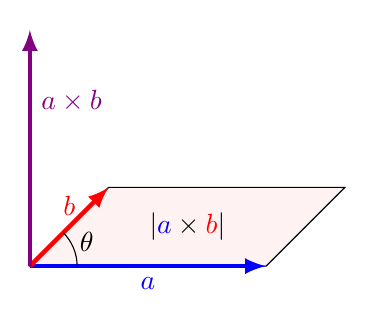
\begin{tikzpicture}
\draw[-,fill=white!95!red](0,0)--(3,0)--(4,1)--(1,1)--cycle;
\node at (2,0.5) {$|\textcolor{blue}{a}\times \textcolor{red}{b}|$};
\draw[ultra thick,-latex,blue](0,0)--(3,0)node[midway,below]{$a$};
\draw[ultra thick,-latex,red](0,0)--(1,1)node[midway,above]{$b$};
\draw[ultra thick,-latex,blue!50!red](0,0)--(0,3)node[pos=0.7,right]{$a\times b$};
\draw (0.6,0) arc [start angle=0,end angle=45,radius=0.6]
node[pos=0.7,right]{$\theta$};

\end{tikzpicture}
\caption{Paralellogram formed by two vectors}
\end{figure}

\subsection{Definition of a plane}

A plane is two-dimensional surface spanned by two linearly independent vectors. 


\begin{itemize}

\item (1) The normal vector of a plane $\vec{n} = \begin{pmatrix}
	a \\
	b \\
	c
\end{pmatrix}$

\item (2) Let $P_1 = \begin{pmatrix}
	x \\
	y \\
	z
\end{pmatrix}$ be a known vector on the plane.
\item (3) Let $P$ be any vector on the plane.

\item (4) A vector connecting $P_1$ to $P$:  $\vec{p} - \vec{p_1} = \begin{pmatrix}

x-x_1 \\
y-y_1 \\
z-z_1

\end{pmatrix} $

\item (5) The vector $\vec{p} - \vec{p_1}$ and $\vec{n}$ are perpendicular, which means that the dot product is zero. $\begin{pmatrix}

a \\
b \\
c 

\end{pmatrix} \cdot \begin{pmatrix}

x-x_1 \\
y-y_1 \\
z-z_1

\end{pmatrix}  = 0$

\item (7) Calculating the dot product, we get: $a(x-x_1) + b(y-y_1) + c(z-z_1) = 0$

\item (8) Simplifying further: $ax + by + cz - (ax_1+by_1+cz_1)$

\item (9) We wish to write the plane equation in the form : $ax+by+cz+d=0$

\item (10) To acheive our desired form of the equation, we can set the value of our constant $d=-(ax_1+by_1+cz_1)$

\end{itemize}

The plane is defined by the end result of our labour (Karl Marx invoked) is the general equation for a two-dimensional plane in 3D: $$ \begin{cases}

Ax+By+Cz+D=0 \\
D=-(Ax_1+By_1+Cz_1)

\end{cases} $$

\subsection{The distance from a point to a plane}


\begin{comment}
Note to self: I am having a hard time understanding things, I don't really know why. I feel like I am falling behind. 
\end{comment}

The distance from a point $P$ to a plane is the dot product of the normal vector $\vec{n}$ and the vector $\vec{P} - \vec{P_1}$, where P1 is a any point on the plane.

\smallskip

Let us now look at the derivation of the formula:

\begin{itemize}

\item (1) Let the points: $P = \begin{pmatrix}

	x_0 \\
	y_0 \\
	z_0 \\
\end{pmatrix}$ and $P_1 = \begin{pmatrix}

x_p \\
y_p \\
z_p
\end{pmatrix}$, where $P_1$ is a point on the plane. 

\item (2) Let $\vec{n}$ be a normal vector from the plane. Using the equation of plane, we can also write $\vec{n} = A + B + C$


\item (3) Let $d$ be the orthogonal distance (is also the shortest distance) from the point to the plane. 

\item (4) Let $\vec{f}$ be the vector that goes from a point $P_1$ on the plane to the point $P$. This distance is $\| \vec{f} \|$ where, $\vec{f} = | \vec{P} - \vec{P_1} |$. Using the equation of a plane, we can also write: $\vec{f} = (x_0 - x_p) + (y_0 -y_p) + (z_0 - z_p)$

\item (5) The orthogonal distance $d$ from the plane o the point $P$. That is: 

$$ \cos{\theta} = \frac{d}{\| \vec{f} \|} $$ where $\theta$ is the angle between the orthogonal distance $D$ and $\| \vec{f} \|$.

\item (6) This can be rewritten as the dot product of the normal vector $\vec{n}$ from the plane, and the distance $\| \vec{f} \|$

$$ \frac{\| \vec{n} \| \| \vec{f}\| \cos{\theta}}{\|\vec{n}\|}  = \frac{\vec{n} \vec{f}}{\|\vec{n}\|} = d $$


\item (7) Let us look at the equations which describe the vectors $\vec{n}$ and $\vec{f}$, and what their dot product is:
$$\frac{\vec{n} \cdot \vec{f}}{\| \vec{n} \|}  = \frac{Ax_0 - Ax_p + Ay_0 - Ay_p + Az_0 - Az_p}{\sqrt{A ^2 + B^2 + C^2}} = d$$

Recall now that the terms $-Ax_p-By_p-Cz_p= D$ from the equation described in the definition of a plane. Hence, we can rewrite the formula above as. 


$$\frac{\vec{n} \cdot \vec{f}}{\| \vec{n} \|}  = \frac{Ax_0 + Ay_0 + Az_0 - D}{\sqrt{A ^2 + B^2 + C^2}} = d$$

\end{itemize}

Our hard work has paid off (as it always does) and now we have a formula for the \textbf{shortest} distance from a point to a plane. This derivation concludes the proof of the stated property.
\begin{comment} 
Hopefully, you are satisfied with this derivation :) 
\end{comment}

\section{Matrices}

\subsection{Definition of a matrix}
A matrix is a set of numbers organised in rows and columns. A $m \times n$ matrix has $ m $ rows and $ n $ columns. 

$$
A = \begin{bmatrix}
	a_{11} & a_{12} &. &a_{1n} \\
	a_{21}& a_{22} &. &a_{2n} \\
	. & . & .&  . \\ 
	. & . & .&  . \\
	. & . & .&  . \\
	a_{m1}& a_{m2}&. &a_{mn} \\
	\end{bmatrix}
$$

\subsection{Definition of a product of a matrix and a vector}

The product of a vector and a matrix is only defined if the vector has the same amount of elements as columns in the matrix. In other words, if the matrix $\bold{A}$ is a $m \times n$ matrix and the vector $v$ is a $l$ dimensional vector. The product of the matrix $\bold{\vec{A}}$ and the vector $\vec{v}$ is only defined if $m=l$. The product of a matrix $A$ and a vector $\vec{x}$ is: 

$$A \vec{x} = \begin{bmatrix}
	a_{11} & a_{12} &. &a_{1n} \\
	a_{21}& a_{22} &. &a_{2n} \\
	. & . & .&  . \\ 
	. & . & .&  . \\
	. & . & .&  . \\
	a_{m1}& a_{m2}&. &a_{mn} \\
	\end{bmatrix} \begin{bmatrix}

	x_1 \\
	x_2 \\
	. \\
	.\\
	.\\
	x_n
\end{bmatrix} = \begin{bmatrix}

	a_{11}x_1 + a_{12} x_2 + \dots + a_{1n}x_n \\
	a_{21}x_1 + a_{22} x_2 + \dots + a_{2n}x_n \\ 
	. \\
	. \\
	.\\
	a_{m1}x_1 + a_{m2} x_2 + \dots + a_{mn}x_n \\ 
\end{bmatrix}
$$

\section{Null space and column space}

\subsection{Definition of the null space of a matrix}

The null space of a matrix A is the set of vectors that satisfy the homogeneous equation $A \vec{x} = 0$, or alternatively in mathemathical language:  $$N(A)=\{ \vec{x} \in \mathbb{R}^n | A\vec{x} = 0 \}$$ Every matrix has at least the trivial null space, consisting of the zero vector. For non-square or singular matrices, the null space may also include non-zero vectors.

\begin{itemize}
	

\item Reduce the matrix to row-echelon-form. 

\item Notice that there are more unknowns than equations. Write out the reduced-echelon-form matrix in equation form.

\item Solve the equation. 

\item Now you can write the solution as a span of vectors, which is set of all possible linear combinations of your solution.

\end{itemize}


\subsubsection{Connection between null space and linear independence}

For a $n \times n$ matrix that only contains linearly independent columns vectors, the only solution to the the equation of the null space is the zero vector. That is: 

\begin{itemize}


\item (1) If we have a matrix $A =\begin{bmatrix}
	a_{11} & a_{12} &. &a_{1n} \\
	a_{21}& a_{22} &. &a_{2n} \\
	. & . & .&  . \\ 
	. & . & .&  . \\
	. & . & .&  . \\
	a_{m1}& a_{m2}&. &a_{mn} \\
	\end{bmatrix}$
\item (2) We can write each column as a column vector. 
$A =\begin{bmatrix}	
	v_1 \\
	v_2 \\
	. \\
	.\\
	.\\
	v_n
\end{bmatrix}$

\item (3) Solve the equation of a null matrix: $$A\vec{x} = \begin{bmatrix}	
	v_1 \\
	v_2 \\
	. \\
	.\\
	.\\
	v_n
\end{bmatrix}\begin{bmatrix}

	x_1 \\
	x_2 \\
	. \\
	.\\
	.\\
	x_n
\end{bmatrix} = x_1\vec{v_1} + x_2\vec{v_2} + ... + x_n\vec{v_n}= \vec{0}$$ 

\item (4) If the vectors $v_1, v_2 ... v_n$ are linearly independent, the only solution to the equation of a null matrix is the zero vector. That is, all of the coefficients $x_1, x_2 ... x_n$ must be zero.


\item For a set of linearly independent column vectors, we observe that the reduced row-echelon form will not have any free variables. That is only ones in the diagonals with zeros everywhere else. So it will always look like: $$\begin{bmatrix}
	1 & 0 &. & . &0 \\
	0 & 1 &. & . &0 \\
	. &. & . &. &.  \\
	. &. & . &. &. \\
	. &. & . &. &. \\
    0&  0& . &. &1 \\ 

	\end{bmatrix}$$
	
\item If the null space is more than just the zero-vector the set of the columns vectors is a linearly dependent set. 
\end{itemize}

\subsection{Definition of a column space}

For a $m \times n$ matrix $A$, the column space is the span of the column vectors of $A$, that is:


\begin{itemize}

\item $A =\begin{bmatrix}	
	v_1 \\
	v_2 \\
	. \\
	.\\
	.\\
	v_n
 \end{bmatrix} \text{,where } \vec{v_1}, \vec{v_2} ... \vec{v_n} \in \mathbb{R} ^n \Rightarrow \text{Col}(A) = \text{span}(\vec{v_1}, \vec{v_2} ... \vec{v_n})$

\end{itemize}

\subsection{Example: Finding the null space and the column space basis}



Let $A = \begin{bmatrix}

1 & 1 & 1 & 1 \\
2 & 1 & 4 & 3 \\
3 & 4 & 1 & 2 


\end{bmatrix} $. Find the null space and the basis of the column space .


\begin{itemize}

\item The null space: $A\vec{x}=0$ 

\item Let us write the matrix in reduced-row echelon form. 



$$A = \begin{bmatrix}

1 & 1 & 1 & 1\\ 
2 & 1 & 4 & 3 \\
3 & 4 & 1 & 2 \\

\end{bmatrix} $$

$R_1 \Rightarrow 2R_2 - R_1$

$$A = \begin{bmatrix}

1 & 1 & 1 & 1\\ 
0 & 1 & -2 & -1 \\
3 & 4 & 1 & 2 \\

\end{bmatrix} $$

$R_3 \Rightarrow R_3 - 3R_1 $

$$A = \begin{bmatrix}

1 & 0 & 3 & 2\\ 
0 & 1 & -2 & -1 \\
0 & 1 & -2 & -1 \\

\end{bmatrix} $$

$R_3 \Rightarrow R_3-R_2$

$$A = \begin{bmatrix}

1 & 0 & 3 & 2\\ 
0 & 1 & -2 & -1 \\
0 & 0 & 0 & 0 \\

\end{bmatrix} $$

\item Write the row-reduced echelon form to an augmented matrix to find the null space.

$$A\vec{x} = \begin{bmatrix}

1 & 0 & 3 & 2\\ 
0 & 1 & -2 & -1 \\
0 & 0 & 0 & 0 \\

\end{bmatrix}\begin{bmatrix}

x_1 \\
x_2 \\
x_3 \\
x_4

\end{bmatrix} = \begin{bmatrix}

0 \\
0 \\
0 \\
0

\end{bmatrix}$$

\item Now we can write the matrix in the form of system of equations.

\begin{center}

$\begin{cases}


x_1 + 3x_3 + 2x_4 = 0 \Rightarrow x_1 = -3x_3 - 2x_4 \\
4x_2 - 2x_3 -x_4 = 0 \Rightarrow x_2 = 2x_3 + x_4
\end{cases}$

\item $x_3$ is a "free variable", meaning it can be set to anything.

\item The null space is all linear combinations of the all the valid solutions: 

$ \text{null(A)} = \text{null(rref(A))} = \begin{pmatrix}

x_1 \\
x_2 \\
x_3 \\
x_4 

\end{pmatrix} = x_3 \begin{pmatrix}

-3 \\
2 \\
1 \\
0

\end{pmatrix} + x_4 \begin{pmatrix}

-2 \\
1 \\
0 \\
1

\end{pmatrix}$ 

$$ =\text{span(}\begin{pmatrix}

-3 \\
2 \\
1 \\
0

\end{pmatrix}, \begin{pmatrix}

-2 \\
1 \\
0 \\
1

\end{pmatrix})$$
\end{center}

\item The column space is the span of the column vectors: 

$$\text{Col(A)=span(} \begin{bmatrix}

1 \\ 2 \\ 3 



\end{bmatrix}, \begin{bmatrix}

1 \\ 1 \\ 4 



\end{bmatrix}, \begin{bmatrix}

1 \\ 4 \\ 1 



\end{bmatrix}, \begin{bmatrix}

1 \\ 3 \\ 2 



\end{bmatrix})$$





\item To find the basis of the column space. Ask:

(1) Are the column vectors in $A$ a linearly independent set? 

	\begin{itemize}

	\item Recall that the column vectors are only linearly independent if the null space of $A$ only contains the zero vector, that is:
	 	\begin{itemize}
	 

		\item $\text{null(A)}=\vec{0} \Leftrightarrow$ if the ONLY solution to $A\vec{x} =\vec{0}$  is $\vec{x} = \vec{0}$ 

	 	\end{itemize}
	 	
	 	\item No, the column vectors in A are not a linearly independent set. We known this directly as the null space contains more that only the zero-vector. In other words, column vectors in A are a linearly dependent set. 

	 	

	 \end{itemize}
	
(2) Find the linearly independent column vectors. 


$$x_1 \begin{bmatrix}

1 \\ 2 \\ 3 



\end{bmatrix} + x_2 \begin{bmatrix}

1 \\ 1 \\ 4 



\end{bmatrix} + x_3 \begin{bmatrix}

1 \\ 4 \\ 1 



\end{bmatrix} + x_4 \begin{bmatrix}

1 \\ 3 \\ 2 



\end{bmatrix} = 0$$

Since, $x_3$ is a free variable, it can be set to anything. Let's set it to zero.

$$x_1 \begin{bmatrix}

1 \\ 2 \\ 3 



\end{bmatrix} + x_2 \begin{bmatrix}

1 \\ 1 \\ 4 



\end{bmatrix} + x_4 \begin{bmatrix}

1 \\ 3 \\ 2 



\end{bmatrix} = 0$$

Move $x_4$ to the other side.


$$x_1 \begin{bmatrix}

1 \\ 2 \\ 3 



\end{bmatrix} + x_2 \begin{bmatrix}

1 \\ 1 \\ 4 



\end{bmatrix} = - x_4 \begin{bmatrix}

1 \\ 3 \\ 2 



\end{bmatrix}$$

Let us now set $x_4 = -1$

$$x_1 \begin{bmatrix}

1 \\ 2 \\ 3 



\end{bmatrix} + x_2 \begin{bmatrix}

1 \\ 1 \\ 4 



\end{bmatrix} =  \begin{bmatrix}

1 \\ 3 \\ 2 



\end{bmatrix}$$

Now we can use the equation form to get concrete values for $x_1$ and $x_2$, plug them in to check if the equality holds. Plug in: $x_4 = -1$ and $x_3 = 0$ gives: 


$$\begin{cases}


x_1 = -3x_3 - 2x_4 \\
x_2 = 2x_3 + x_4 

\end{cases}$$


$$\begin{cases}


x_1 = 2\\
x_2 = -1

\end{cases}$$

Put these values back in to check equality: 


$$2 \begin{bmatrix}

1 \\ 2 \\ 3 



\end{bmatrix} -1 \begin{bmatrix}

1 \\ 1 \\ 4 



\end{bmatrix}=\begin{bmatrix}

1 \\ 3 \\ 2 



\end{bmatrix}$$

The equality holds. This means that the set $
\{ \begin{bmatrix}

1\\
2\\
3


\end{bmatrix}, \begin{bmatrix}
1 \\
1 \\
4


\end{bmatrix} \}$ is the basis of the column space of A. This consequentially means that the column space can be rewritten as the span of these linearly independent vectors:

col(A) = span($\begin{bmatrix}

1\\
2\\
3


\end{bmatrix}, \begin{bmatrix}
1 \\
1 \\
4


\end{bmatrix}$)



\end{itemize}

\subsection{Proof: Any subspace basis has same number of elements}

\textbf{Theorem:} Let $A=\{v_1, v_2 ..., v_n\}$ be a basis for a subspace $V$. Any set that spans the subspace $V$ must have \textbf{at least} $n$ elements.


\textbf{Proof by contradiction:}

\begin{itemize}

\item (1) Let's assume that there exists a set $B$ that spans $V$ and has less than $n$ elements. $ B =\{ b_1, b_2 ... b_m \}$ where $m<n$. 

\item (2) Let us now define a new set: $B_1' = B  + \{v_1\}$ 

	\begin{itemize}
	
		\item $B_1' = ¨ \{ v_1, b_1, b_2, ... ,b_m  \}$
	
	\end{itemize}		

This set is linearly dependent since $v_1 \in V$  and the vectors: $b_1, b_2, ... ,b_m$, as per the definition span $V$. In other words, $v_1$ can be written as linear combination of $b_1, b_2, ... ,b_m$, where at least one coefficient is non-zero.

	\begin{itemize}

		\item $v_1 = d_1b_1 + d_2b_2 + d_3b_3 + ... + d_mb_m$
		

	\end{itemize}


\item (3) For at least one non-zero coefficient $d_j \neq 0$, the term $b_j$ can be rewritten as:
 
$$b_j = - \frac{1}{d_j} (d_1b_1 + ... + d_{j-1}b_{j-1} + d_{j+1}b_{j+1} + ... + d_mb_m - v_1)$$
	
	

\item (4) We observe that the vector $b_j$ can be written as a linear combination of the other vectors, and therefore we can omit it and still span V. Let us now define a new set, with slight change in notation. Let us call $b_j = b_1$ and $b_1 = b_j$

	\begin{itemize}
	
		\item $B_1 = \{v_1,b_2,b_3...,b_m\}$

	\end{itemize}


\item (5) Let's define a new set where we add the $a_2$ from the: $B_2' = B_1  + \{a_2\}$ 

	\begin{itemize}
	
		\item $B_2' =  \{ a_1, a_2, b_2, ... ,b_m  \}$
	
	\end{itemize}		

This set is linearly dependent since $a_2 \in V$  and the vectors: $a_1, b_2, ... ,b_m$, as per the definition span $V$. In other words, $a_2$ can be written as linear combination of $a_1, b_2, b_3, ... ,b_m$, where at least one coefficient is non-zero.

	\begin{itemize}

		\item $a_2 = c_1a_1 + c_2b_2 + c_3b_3 + ... + c_mb_m$
		

	\end{itemize}


\item (6) For at least one non-zero coefficient $c_j \neq 0$, the term $b_j$ can be rewritten as:
 
$$b_j = - \frac{1}{c_j} (c_1a_1 + ... + c_{j-1}b_{j-1} + c_{j+1}b_{j+1} + ... + c_mb_m - a_2)$$
	
	
\item (7) We observe that the vector $c_j$ can be written as a linear combination of the other vectors, and therefore we can omit it and still span V. Let us now define a new set, with slight change in notation. Let us call $c_j = b_2$ and $b_2 = c_j$

	\begin{itemize}
	
		\item $B_2 = \{v_1,v_2,b_3...,b_m\}$

	\end{itemize}

\item (8) This process can be repeated and hence new sets can be constructed until all of the elements $b_j$ in the set been replaced by an element from the set $A$. 

This will result in a set, which per definition will span V.

$$B_m = \{ a_1, a_2, a_3, ..., a_m \}$$ 

\item (9) Recall the set $A$ which was the basis of V:

$$ A = \{ a_1,a_2 ... a_m, ..., a_n  \}$$

The existence of the set $B_m$ which spans V which has $m$ elements infers that the set $A$ is linearly dependent since it contains more vectors than the set $B_m$. This is clearly a  \textbf{contradiction} because it implies that $A$ is not linearly independent and hence not a basis for V. Hence proved. There cannot exist a spanning set $B$ which has fewer elements than the basis $A$ for V. 


\end{itemize}




Watch: \url{https://www.youtube.com/watch?time_continue=1088&v=Zn2K8UIT8r4&embeds_referring_euri=https%3A%2F%2Fwww.khanacademy.org%2F&embeds_referring_origin=https%3A%2F%2Fwww.khanacademy.org}


\section{Properties of a matrix}

\subsection{Definition of dimension}
 
The dimension of a matrix often denoted as dim is the number of elements (also know as the cardinality) of any basis of a subspace. Every basis of a subspace has the same dimension, or in simpler terms, every basis of a subspace has the same number of elements.

\smallskip

\begin{itemize}

\item (1) Let $V$ be a subspace

\item (2) Let $A = \{ a_1, a_2,...,a_n\}$ be a basis of $V$.

\item (3) The dimension of V is: dim(V) = $n$


\end{itemize}


\subsection{Dimension of the null space}

The dimension of the null space of a matrix \( A \) refers to the number of free variables in the system \( A\vec{x} = 0 \), which corresponds to the number of non-pivot columns in the reduced row-echelon form (RREF) of \( A \).


\begin{itemize}

\item (1) Given the matrix 
\[
A = \begin{pmatrix}
1 & 2 & -1 & 3 \\
2 & 4 & -2 & 6 \\
-1 & -2 & 1 & -3
\end{pmatrix},
\]
we want to determine the dimension of the null space of \( A \).

\item (2) Reduce \( A \) to its RREF

Perform Gaussian elimination to obtain the RREF of \( A \):
\[
\text{RREF}(A) = \begin{pmatrix}
1 & 2 & -1 & 3 \\
0 & 0 & 0 & 0 \\
0 & 0 & 0 & 0
\end{pmatrix}.
\]

\item (3) Identify pivot and free variables

-Pivot columns: Columns 1 (first) is a pivot column because it contains the leading 1 in its row.
- Non-pivot columns: Columns 2, 3, and 4 do not have pivots.

\item (4) Determine the dimension of the null space

The number of non-pivot columns is 3. Therefore, the dimension of the null space of \( A \) is 3.

\end{itemize}

The dimension of the null space of a matrix \( A \) is equal to the number of non-pivot columns in its reduced row-echelon form. In this example, the null space has a dimension of 3, meaning that the solution set to \( A\vec{x} = 0 \) has 3 free variables, and hence a 3-dimensional null space.

\subsection{Dimension of the column space or rank}

The dimension of a column space of a matrix, also called the \textit{rank} is the number of pivot columns in the reduced row-echelon form of $A$.

\begin{itemize}


\item (1) Let $A$: $\begin{bmatrix}
1 & 0 & -1 & 0 & 4 \\
0 & 1 & 2 & 0  & 1 \\
0 & 0 & 0 & 1  & -3 \\ \end{bmatrix}$

\item (2) The column space is: span$( \begin{pmatrix}

1 \\ 0 \\ 0

\end{pmatrix}$ $\begin{pmatrix}

0 \\ 1 \\ 0

\end{pmatrix}$ $\begin{pmatrix}

1 \\ 2 \\ 0

\end{pmatrix}$ $\begin{pmatrix}

0 \\ 0 \\ 1

\end{pmatrix}$ $\begin{pmatrix}

4 \\ 1 \\ -3

\end{pmatrix})$

\item (3) Perform elementary row operation to get the RREF form. In this case, the matrix is already in RREF. 

\item (4) The column space is the set of the basis vectors of $A$ vectors, that is the set of linearly independent vectors in $A$: \begin{center}

 Col(A) = span($\begin{pmatrix}

1 \\ 0 \\ 0

\end{pmatrix}$ $\begin{pmatrix}

0 \\ 1 \\ 0

\end{pmatrix}$ $\begin{pmatrix}

0 \\ 0 \\ 1

\end{pmatrix}$) \end{center}

\item (5) The dimension of the column space dim(Col(A)) = 3 or rank(A) = 3.

\end{itemize}

\section{Linear Transformation}

\subsection{Definition of a linear transformation}
A linear transformation is a \textbf{function} $T: V \to W$ between two vector spaces $V$ and $W$ if it satisfies the following two properties for all vectors $\mathbf{u}, \mathbf{v} \in V$.

\begin{enumerate}
    \item Additivity: $T(\mathbf{u} + \mathbf{v}) = T(\mathbf{u}) + T(\mathbf{v})$.
    \item Homogeneity: $T(c \mathbf{u}) = c T(\mathbf{u})$.
\end{enumerate}

A transformation is said to be linear \textbf{if and only if} it satisfies these criterion.



\subsection{Properties of Linear Transformations}
\subsubsection{Preservation of the Zero Vector}
\textbf{Property:} A linear transformation maps the zero vector in $V$ to the zero vector in $W$:
\[
T(\mathbf{0}) = \mathbf{0}.
\]

\textbf{Proof:}
\begin{align*}
    T(\mathbf{0}) &= T(\mathbf{0} + \mathbf{0}) \quad \text{(since $\mathbf{0} + \mathbf{0} = \mathbf{0}$)} \\
    &= T(\mathbf{0}) + T(\mathbf{0}) \quad \text{(by additivity)}.
\end{align*}
Subtracting $T(\mathbf{0})$ from both sides gives:
\[
T(\mathbf{0}) = \mathbf{0}.
\]

\subsubsection{Preservation of Scalar Multiplication}
\textbf{Property:} For any scalar $c \in \mathbb{R}$ and vector $\mathbf{v} \in V$,
\[
T(c \mathbf{v}) = c T(\mathbf{v}).
\]

\textbf{Proof:} This property follows directly from the homogeneity property in the definition of a linear transformation.

\subsection{Linearity}
\textbf{Property:} For any $\mathbf{u}, \mathbf{v} \in V$ and $a, b \in \mathbb{F}$,
\[
T(a \mathbf{u} + b \mathbf{v}) = a T(\mathbf{u}) + b T(\mathbf{v}).
\]

\textbf{Proof:}
By additivity and homogeneity, we compute:
\begin{align*}
    T(a \mathbf{u} + b \mathbf{v}) &= T(a \mathbf{u}) + T(b \mathbf{v}) \quad \text{(by additivity)} \\
    &= a T(\mathbf{u}) + b T(\mathbf{v}) \quad \text{(by homogeneity)}.
\end{align*}

\subsection{Uniqueness of Linear Transformations}
\textbf{Property:} If $T: V \to W$ is linear, then $T$ is completely determined by its action on a basis of $V$.

\textbf{Proof:}
Let $\{\mathbf{v}_1, \mathbf{v}_2, \dots, \mathbf{v}_n\}$ be a basis of $V$. Any vector $\mathbf{v} \in V$ can be written as a linear combination:
\[
\mathbf{v} = c_1 \mathbf{v}_1 + c_2 \mathbf{v}_2 + \dots + c_n \mathbf{v}_n.
\]
By linearity,
\[
T(\mathbf{v}) = T(c_1 \mathbf{v}_1 + c_2 \mathbf{v}_2 + \dots + c_n \mathbf{v}_n) = c_1 T(\mathbf{v}_1) + c_2 T(\mathbf{v}_2) + \dots + c_n T(\mathbf{v}_n).
\]
Thus, $T$ is fully determined by $T(\mathbf{v}_1), T(\mathbf{v}_2), \dots, T(\mathbf{v}_n)$.

\subsection{Definition of addition of linear transformations}

For any linear transformations: $S: \mathbb{R}^n \to \mathbb{R}^m$ and $T:\mathbb{R}^n \to \mathbb{R}^m$ the addition of linear transformation $(S+T)$ is defined as: 
$$\boxed{(S+T)(\vec{x}) = S(\vec{x}) + T(\vec{x})}$$. 

where the linear transformations: $S+T: \mathbb{R}^n \to \mathbb{R}^m$

\textbf{Special note:} Addition of linear transformations is only defined for matrices with the same dimension. This follows directly from the definition of the addition of matrices. 

\smallskip

\textbf{Further explanation:} For any linear transformations: $S(\vec{x}) = \underset{m \times n}{A}\vec{x}$ and $T(\vec{x}) = \underset{m \times n}{B} \vec{x}$. The sum of the transformations $(S+T)\vec{x}$ can be written as: $S(\vec{x}) + T(\vec{x})$ which gives: $\underset{m \times n}{A}\vec{x} + \underset{m \times n}{B}\vec{x}$.

\smallskip

$$\underset{m \times n}{A} = \begin{bmatrix}

\vec{a_1} & \vec{a_2} &. &. &.  &\vec{a_n}

\end{bmatrix} \quad \text{and} \quad \underset{m \times n}{B} = \begin{bmatrix}

\vec{b_1} & \vec{b_2} &. &. &.  &\vec{b_n}

\end{bmatrix}$$

and any vector 

$$\vec{x} = \begin{bmatrix}

x_1 \\ x_2 \\. \\. \\.  \\x_n

\end{bmatrix}$$

The sum of the linear transformations can be written:

$$\underset{m \times n}{A}\vec{x} + \underset{m \times n}{B}\vec{x} = \begin{bmatrix}

\vec{a_1} & \vec{a_2} &. &. &.  &\vec{a_n}

\end{bmatrix} \begin{bmatrix}

\vec{b_1} & \vec{b_2} &. &. &.  &\vec{b_n}

\end{bmatrix}$$

$$=x_1a_1 + x_2a_2 + ... + x_na_n + x_1b_1 + x_2b_2 + ... + x_nb_n$$

$$=x_1(a_1+b_1) + x_2(a_2+b_2) + ... + x_n(a_n+b_n)$$

$$= \begin{bmatrix}

x_1 \\ x_2 \\. \\. \\.  \\x_n

\end{bmatrix} \begin{bmatrix}

\vec{a_1} + \vec{b_1}  & \vec{a_2} + \vec{b_2} &. &. &.  &\vec{a_n} + \vec{b_n}

\end{bmatrix}$$

Hence, proved. $(S+T)(\vec{x}) = S(\vec{x}) + T(\vec{x})$ 

\subsection{Definition of scalar multiplications of linear transformations}

For any linear transformation: $S: \mathbb{R}^n \to \mathbb{R}^m$ the scalar multiplication of a linear transformation $(cS)(\vec{x}) = c(S(\vec{x}))$ is defined as: 
$$\boxed{(cS)(\vec{x}) = c(S(\vec{x}))}$$

where the linear transformations: $cS: \mathbb{R}^n \to \mathbb{R}^m$

\smallskip

\textbf{Further explanation:} For any linear transformation $S: \mathbb{R}^n \to \mathbb{R}^m$, it follows directly from the \textit{properties of linear transformations} that is possible to write it as a scalar times the linear transformation. That is: 


\smallskip 

$$S(\vec{x}) = \underset{m \times n}{A} \vec{x} \quad \text{where} \quad \underset{m \times n}{A} = \begin{bmatrix}

\vec{a_1} & \vec{a_2} &. &. &.  &\vec{a_n}

\end{bmatrix}$$

Multiplication with a scalar gives: 
$$c(S(\vec{x})) = c\underset{m \times n}{A}\vec{x}$$

$$=c(\vec{x_1}a_1 + \vec{x_2}a_2 + ... + \vec{x_n}a_n)$$

Distributing $c$ gives: 

$$=c\vec{x_1}a_1 + c\vec{x_2}a_2 + ... + c\vec{x_n}a_n$$

Writing the multiplication in terms of a matrix results in: 

$$=\begin{bmatrix}

c\vec{a_1} & c\vec{a_2} &. &. &. &c\vec{a_n}

\end{bmatrix} \begin{bmatrix}

x_1 \\ x_2 \\. \\. \\.  \\x_n
\end{bmatrix}$$

Notice that the first matrix is exactly the same as: $c\underset{m \times n}{A}$. Therefore we conclude proof by asserting that: $(cS)(\vec{x}) = c(S(\vec{x}))$


\subsection{Proof: Matrix vector products are linear transformations}

\textbf{Property:} For any matrix $\underset{m \times n}{A} = \begin{bmatrix}


\vec{v_1} , \vec{v_2} ... , \vec{v_n}

\end{bmatrix}$ and any vector $\vec{x} = \begin{bmatrix}

x_1 \\ x_2 \\. \\. \\. \\ x_n

\end{bmatrix}$ \bigskip

 The matrix vector product is: $$A\vec{x} = \begin{bmatrix}


\vec{v_1} , \vec{v_2} ... , \vec{v_n} 

\end{bmatrix} \begin{bmatrix}

x_1 \\ x_2  \\. \\. \\. \\ x_n

\end{bmatrix} = x_1\vec{v_1} + x_2\vec{v_2} + ... + x_n\vec{v_n}$$

\textbf{Recall:} The two requirements for a transformation to be linear are additivity: $T(\vec{a} + \vec{b}) = T(\vec{a}) + T(\vec{b})$ and homogeneity: $T(c\vec{a}) = cT(\vec{a})$. 

\bigskip

We need to prove that matrix vector products meet these two criterion. \begin{center}


For any vectors $\vec{a} = \begin{bmatrix}

a_1 \\ a_2 \\. \\. \\. \\a_n

\end{bmatrix}$   and $\vec{b} = \begin{bmatrix}

b_1 \\b_2 \\.\\. \\. \\b_n 

\end{bmatrix} $

\end{center} 

\begin{itemize}

\item \textbf{Question:} Are matrix vectors products additive? In other words, is $A(\vec{a} + \vec{b}) = A(\vec{a}) + A(\vec{b})$? Let's investigate.

$$\underset{m \times n}{A}(\vec{a} + \vec{b}) = \underset{m \times n}{A}\begin{bmatrix}

a_1 + b_1 \\
a_2 + b_2 \\
.\\
.\\
.\\
a_n + b_n
\end{bmatrix}$$

$$=(a_1+b_1)\vec{v_1}+(a_2+b_2)\vec{v_2}+...+(a_n+b_n)\vec{v_n}$$
$$=\color{blue} (a_1\vec{v_1} + a_2\vec{v_2} + ... + a_n\vec{v_n}) + \color{red} (b_1\vec{v_1} + b_2\vec{v_2} + ... + b_n\vec{v_n})$$


Observe that the terms: $\color{blue} a_1\vec{v_1} + a_2\vec{v_2} + ... + a_n\vec{v_n}$ are equal to $A\vec{a}$, likewise the terms $\color{red} (b_1\vec{v_1} + b_2\vec{v_2} + ... + b_n\vec{v_n})$ are equal to $A\vec{b}$. Hence: $$\underset{m \times n}{A}(\vec{a} + \vec{b}) = \underset{m \times n}{A}\vec{a} + \underset{m \times n}{A}\vec{b} $$

\textbf{Answer:} Yes. Matrix vector products are additive. 

\item \textbf{Question:} Are matrix vector products homogeneous? In other words, is 
$\underset{m \times n}{A}(c\vec{a}) = c\underset{m \times n}{A}\vec{a}$? Let's investigate this spooky territory. 

$$ A(c\vec{a})=\begin{bmatrix}


\vec{v_1} , \vec{v_2} \dots , \vec{v_n}

\end{bmatrix} \begin{bmatrix}
ca_1 \\ ca_2 \\. \\. \\. \\ca_n 
\end{bmatrix} = ca_1\vec{v_1} + ca_2\vec{v_2} + ... + ca_n\vec{v_n}$$ 

$$= \color{purple}c(a_1\vec{v_1} + a_2\vec{v_2} + ... + a_n\vec{v_n})$$

Observe that the terms: $\color{purple}c(a_1\vec{v_1} + a_2\vec{v_2} + ... + a_n\vec{v_n})$ are equal to $cA\vec{a}$. Hence: $\color{purple}c(a_1\vec{v_1} + a_2\vec{v_2} + ... + a_n\vec{v_n}) = \normalcolor cA\vec{a}$

\textbf{Answer:} Yes. Matrix vector products are homogenous.
\begin{comment} 
(I am going insane while writing this) (2025.11.05 - I can corroborate that I did in fact go insane while writing this.)
\end{comment} 

\end{itemize}


\subsection{Proof: Any matrix can be written in terms of the identity matrix}

\textbf{Property:} Any matrix multiplied with the identity matrix (a square matrix) returns the same matrix. That is: $\underset{n \times n}{I_n}\vec{x} = \vec{x}$ where  $\vec{x} \in \mathbb{R}^n$, where the vectors $\{ \vec{e_1}, \vec{e_2} , ... , \vec{e_3}\}$ are the standard basis for $\mathbb{R}^n$. That is: 

$$\underset{n \times n}{I_n} = \begin{bmatrix}

1 & 0 & 0 &. &. &. &. &0 \\
0 & 1 & 0 &. &. &. &. &0 \\
0 & 0 & 1 &. &. &. &. &0 \\
0 & 0 & 0 &1 &. &. &. &0 \\
0 & 0 & 0 &. &1 &. &. &0 \\
0 & 0 & 0 &. &. &1 &. &0 \\
0 & 0 & 0 &. &. &. &1 &0 \\

\end{bmatrix} $$

The identity matrix can be written as it's column vectors: 

$$\underset{n \times n}{I_n} = \begin{bmatrix}

\vec{e_1}, & \vec{e_2}, &. &. &. &\vec{e_n}

\end{bmatrix} $$

Any vector $\vec{x} = \begin{bmatrix}


a_1 \\ a_2 \\. \\. \\. \\a_n
\end{bmatrix}$ can be as a matrix vector product with the identity matrix and the result will be the vector itself. 


$$I_n\vec{x}= a_1\vec{e_1} + a_2\vec{e_2} + ... + a_n\vec{e_n} $$
$$=\begin{bmatrix}

a_1 \\ 0 \\. \\. \\. \\0

\end{bmatrix} + \begin{bmatrix}

0 \\ a_2 \\. \\. \\. \\0

\end{bmatrix} + ... + \begin{bmatrix}

0 \\ 0 \\. \\. \\. \\a_n

\end{bmatrix} = \begin{bmatrix}


a_1 \\ a_2 \\. \\. \\. \\a_n
\end{bmatrix} $$

$$=\vec{x}$$

Notice that each term is an element in the vector $\vec{x}$. 

\subsection{Proof: Any linear transformation can be written as a matrix vector product}

This proof is equivalent to the previous two proofs combined, but presented in the reverse order. 


\textbf{Property:} Any linear transformation $T:\mathbb{R}^n \to \mathbb{R}^m$ for any vector $\vec{x}$ can be written as the product of the vector multiplied by the matrix containing the transformed basis vectors for $\mathbb{R}^n$.

\textbf{Proof:}

\begin{itemize}

\item Any vector $\vec{x}$ can be written as the product of the identity matrix times itself. That is $\underset{n \times n}{I_n}\vec{x} = \vec{x} \Leftrightarrow \vec{x} = a_1\vec{e_1} + a_2\vec{e_2} + ... + a_n\vec{e_n} = \vec{x}$ 

\item A linear transformation of a vector can be written as: $T(\vec{x}) = T(a_1\vec{e_1} + a_2\vec{e_2} + ... + a_n\vec{e_n})$ 

\item The additive property of linear transformations gives: $T(\vec{x}) = a_1T(e_1) + a_2 T(e_2) + ... + a_nT(e_n)$

\end{itemize}

\smallskip

The transformation can be written as the: $$ T(\vec{x}) = \begin{bmatrix}

T(\vec{e_1}) & T(\vec{e_2}) &. &. &. &T(\vec{e_n})

\end{bmatrix} \begin{bmatrix}
x_1 \\ x_2 \\. \\. \\. \\x_n \\

\end{bmatrix}$$



\subsection{Examples of Linear Transformations}

\subsubsection{Scaling}

\begin{itemize}

\item Uniform Shrinking: A transformation that reduces all vectors' lengths by half:
\[
T(\vec{x}) = \begin{bmatrix} 0.5 & 0 \\ 0 & 0.5 \end{bmatrix} \vec{x}
\]
If \( \vec{x} = \begin{bmatrix} x_1 \\ x_2 \end{bmatrix} \), then
\[
T(\vec{x}) = \begin{bmatrix} 0.5x_1 \\ 0.5x_2 \end{bmatrix}
\]

\item Non-Uniform Scaling: A transformation that doubles the \( x \)-coordinate but triples the \( y \)-coordinate:
\[
T(\vec{x}) = \begin{bmatrix} 2 & 0 \\ 0 & 3 \end{bmatrix} \vec{x}
\]
If \( \vec{x} = \begin{bmatrix} x_1 \\ x_2 \end{bmatrix} \), then
\[
T(\vec{x}) = \begin{bmatrix} 2x_1 \\ 3x_2 \end{bmatrix} \]

\end{itemize}

\subsubsection{Reflection}

\begin{itemize}


\item Reflection Across the Line \( y = -x \):
\[
T(\vec{x}) = \begin{bmatrix} 0 & -1 \\ -1 & 0 \end{bmatrix} \vec{x}
\]
If \( \vec{x} = \begin{bmatrix} x_1 \\ x_2 \end{bmatrix} \), then
\[
T(\vec{x}) = \begin{bmatrix} -x_2 \\ -x_1 \end{bmatrix}
\]

\item Reflection Across a Plane in 3D (e.g., Plane \( z = 0 \)):

 For \( T:\mathbb{R}^3 \to \mathbb{R}^3 \), the reflection matrix is:
\[
T(\vec{x}) = \begin{bmatrix} 1 & 0 & 0 \\ 0 & 1 & 0 \\ 0 & 0 & -1 \end{bmatrix} \vec{x}
\]
If \( \vec{x} = \begin{bmatrix} x_1 \\ x_2 \\ x_3 \end{bmatrix} \), then
\[
T(\vec{x}) = \begin{bmatrix} x_1 \\ x_2 \\ -x_3 \end{bmatrix}
\]

\end{itemize}

\subsubsection{Definition of a projection}

A projection is a linear transformation that maps a vector onto a subspace (for example: a line or plane) such that the resulting vector lies entirely within that subspace. Mathematically, a projection $T$ satisfies the property $T^2=T$, meaning applying the transformation twice has the same effect as applying it once.


\subsubsection{Projection}
\begin{itemize}

\item Projection Onto a Plane in 3D (e.g., Plane \( z = 0 \)):
\[
T(\vec{x}) = \begin{bmatrix} 1 & 0 & 0 \\ 0 & 1 & 0 \\ 0 & 0 & 0 \end{bmatrix} \vec{x}
\]
If \( \vec{x} = \begin{bmatrix} x_1 \\ x_2 \\ x_3 \end{bmatrix} \), then
\[
T(\vec{x}) = \begin{bmatrix} x_1 \\ x_2 \\ 0 \end{bmatrix}
\]

\item Orthogonal Projection Onto a Subspace in 2D (e.g., Line \( y = 2x \)):  
Let \( \vec{u} = \begin{bmatrix} 1 \\ 2 \end{bmatrix} \) be a direction vector. Normalize \( \vec{u} \) to get \( \vec{u} = \frac{1}{\sqrt{5}} \begin{bmatrix} 1 \\ 2 \end{bmatrix} \). The projection matrix is:
\[
T(\vec{x}) = \vec{u}\vec{u}^\top = \frac{1}{5} \begin{bmatrix} 1 & 2 \\ 2 & 4 \end{bmatrix}
\]


\end{itemize}

\subsubsection{Rotation}

\begin{itemize}

\item Rotation by 45 degrees counter-clockwise:
\[
T(\vec{x}) = \begin{bmatrix} \cos 45^\circ & -\sin 45^\circ \\ \sin 45^\circ & \cos 45^\circ \end{bmatrix} = \frac{1}{\sqrt{2}} \begin{bmatrix} 1 & -1 \\ 1 & 1 \end{bmatrix}
\]

\item 3D Rotation About the \( z \)-Axis by 90 Degrees:


For \( T:\mathbb{R}^3 \to \mathbb{R}^3 \), the rotation matrix is:
\[
T(\vec{x}) = \begin{bmatrix} 0 & -1 & 0 \\ 1 & 0 & 0 \\ 0 & 0 & 1 \end{bmatrix} \vec{x}
\]
If \( \vec{x} = \begin{bmatrix} x_1 \\ x_2 \\ x_3 \end{bmatrix} \), then
\[
T(\vec{x}) = \begin{bmatrix} -x_2 \\ x_1 \\ x_3 \end{bmatrix}
\]
\end{itemize}

	

\subsubsection{Definition of a composition}

A composition of linear transformations is defined as the composition of the functions which describe the linear transformations. In other words, the composition of linear transformations is simply just a composition of functions. 

\smallskip 

The composition of two functions $f$ and $g$, denoted as $(f\circ g)(x)$, is a new function formed by applying $g$ first to an input $x$, and then applying $f$ to the result of $g(x)$. That is:

$$(f\circ g)(x)=f(g(x))$$

\subsubsection{Proof: Composition of linear transformations is also a linear transformation}

\textbf{Property:} For any linear transformations $S: X \to Y$ and $T: Y \to Z$, where $x\subseteq \mathbb{R}^n$, $Y\subseteq \mathbb{R}^m$ and $Z\subseteq \mathbb{R}^l$. Let $S(\vec{x}) = \underset{m \times n}{A}\vec{x}$ and $T(\vec{x}) = \underset{lxm}{B}\vec{x}$. The composition $T \circ S : X \to Z$ is $T(S(\vec{x}))$ is also a linear transformation.

\smallskip

\textbf{Proof:} A transformation \( G \) is linear if for all \( \vec{x}, \vec{y} \in \mathbb{R}^n \) and scalars \( c \in \mathbb{R} \), the properties of additivity and homogeneity hold. 

Let \( S: \mathbb{R}^n \to \mathbb{R}^m \) and \( T: \mathbb{R}^m \to \mathbb{R}^l \) be linear transformations. We need to show that \( S \circ T (\vec{x}) = S(T(\vec{x})) \) satisfies both properties:

\smallskip

\textbf{1. Additivity:}
\[
(S \circ T)(\vec{x} + \vec{y}) = S(T(\vec{x} + \vec{y}))
\]
Since \( S \) is linear:
\[
S(\vec{x} + \vec{y}) = S(\vec{x}) + S(\vec{y})
\]
Applying \( T \), and since \( T \) is linear:
\[
T(S(\vec{x}) + S(\vec{y})) = T(S(\vec{x})) + T(S(\vec{y}))
\]
Thus:
\[
(S \circ T)(\vec{x} + \vec{y}) = (S \circ T)(\vec{x}) + (S \circ T)(\vec{y})
\]

\textbf{2. Homogeneity:}
\[
(S \circ T)(c\vec{x}) = S(T(c\vec{x}))
\]
Since \( S \) is linear:
\[
S(c\vec{x}) = cS(\vec{x})
\]
Applying \( T \), and since \( T \) is linear:
\[
T(cS(\vec{x})) = cT(S(\vec{x}))
\]
Thus:

\[
\boxed{
(S \circ T)(c\vec{x}) = c(S \circ T)(\vec{x})}
\]

Hence, proved. We can safely conclude that since both additivity and homogeneity are satisfied, \( T_2 \circ T_1 \) is a linear transformation.


\subsection{Examples of matrix products in compositions of linear transformations}

To understand the relationship between matrix products and compositions of linear transformations, consider the following examples:

\subsubsection{Example 1: Scaling and Rotation}

Suppose we have two linear transformations in \( \mathbb{R}^2 \):
\begin{itemize}
    \item A scaling transformation \( S \) defined by \( S(x, y) = (2x, 3y) \), represented by the matrix
    \[
    S = \begin{bmatrix}
    2 & 0 \\
    0 & 3
    \end{bmatrix}.
    \]
    \item A rotation transformation \( R \) of \( 90^\circ \) counterclockwise, represented by the matrix
    \[
    R = \begin{bmatrix}
    0 & -1 \\
    1 & 0
    \end{bmatrix}.
    \]
\end{itemize}

The composition \( R \circ S \) applies the scaling transformation first, followed by the rotation. The combined effect can be represented as the product of the matrices:
\[
RS = \begin{bmatrix}
0 & -1 \\
1 & 0
\end{bmatrix}
\begin{bmatrix}
2 & 0 \\
0 & 3
\end{bmatrix} = \begin{bmatrix}
0 & -3 \\
2 & 0
\end{bmatrix}.
\]
This resulting matrix represents the combined transformation.

\subsubsection{Example 2: Shear and Reflection}

Consider two transformations in \( \mathbb{R}^2 \):
\begin{itemize}
    \item A shear transformation \( H \) along the \( x \)-axis, defined by \( H(x, y) = (x + y, y) \), represented by
    \[
    H = \begin{bmatrix}
    1 & 1 \\
    0 & 1
    \end{bmatrix}.
    \]
    \item A reflection transformation \( F \) across the \( y \)-axis, represented by
    \[
    F = \begin{bmatrix}
    -1 & 0 \\
    0 & 1
    \end{bmatrix}.
    \]
\end{itemize}

The composition \( F \circ H \) applies the shear first, followed by the reflection. The matrix product is:
\[
FH = \begin{bmatrix}
-1 & 0 \\
0 & 1
\end{bmatrix}
\begin{bmatrix}
1 & 1 \\
0 & 1
\end{bmatrix} = \begin{bmatrix}
-1 & -1 \\
0 & 1
\end{bmatrix}.
\]
This matrix represents the combined transformation.

\subsubsection{Example 3: 3D Transformation - Rotation and Translation}

In \( \mathbb{R}^3 \), consider:
\begin{itemize}
    \item A rotation about the \( z \)-axis by \( \theta \):
    \[
    R_z = \begin{bmatrix}
    \cos\theta & -\sin\theta & 0 \\
    \sin\theta & \cos\theta & 0 \\
    0 & 0 & 1
    \end{bmatrix}.
    \]
    \item A translation (using homogeneous coordinates) \( T \):
    \[
    T = \begin{bmatrix}
    1 & 0 & 0 & a \\
    0 & 1 & 0 & b \\
    0 & 0 & 1 & c \\
    0 & 0 & 0 & 1
    \end{bmatrix}.
    \]
\end{itemize}

The composition \( T \circ R_z \) applies the rotation first, then the translation. The product is:
\[
TR_z = \begin{bmatrix}
1 & 0 & 0 & a \\
0 & 1 & 0 & b \\
0 & 0 & 1 & c \\
0 & 0 & 0 & 1
\end{bmatrix}
\begin{bmatrix}
\cos\theta & -\sin\theta & 0 & 0 \\
\sin\theta & \cos\theta & 0 & 0 \\
0 & 0 & 1 & 0 \\
0 & 0 & 0 & 1
\end{bmatrix} = \begin{bmatrix}
\cos\theta & -\sin\theta & 0 & a \\
\sin\theta & \cos\theta & 0 & b \\
0 & 0 & 1 & c \\
0 & 0 & 0 & 1
\end{bmatrix}.
\]
´
This matrix describes the combined transformation.

\smallskip

These examples illustrate how matrix multiplication encapsulates the sequential application of linear transformations. By analyzing the resulting matrices, we can gain insight into the combined effects of these transformations.

\subsection{Proof: Compositions of linear transformations is associative}

\textbf{Property:} The composition of linear transformations is associative, a property which follows directly from the associative property of matrix products. For linear transformations \(T_1\), \(T_2\), and \(T_3\): 
\[
(T_1 \circ T_2) \circ T_3 = T_1 \circ (T_2 \circ T_3).
\]

\textbf{Proof:}
Let \(V\), \(W\), and \(X\) be vector spaces, and let \(T_1: W \to X\), \(T_2: V \to W\), and \(T_3: U \to V\) be linear transformations. For any vector \(u \in U\), we consider the composition of these transformations:

\begin{itemize}


\item (1) Compute \(T_3(u) \in V\).
\item (2) Apply \(T_2\) to obtain \(T_2(T_3(u)) \in W\).
\item (3) Apply \(T_1\) to obtain \(T_1(T_2(T_3(u))) \in X\).


\end{itemize}

Now, we analyze the associativity in two ways:

\begin{itemize}


\item 1. \((T_1 \circ T_2) \circ T_3(u)\):
\[
(T_1 \circ T_2)(T_3(u)) = T_1(T_2(T_3(u))).
\]

\item  2. \(T_1 \circ (T_2 \circ T_3)(u)\):
\[
T_1((T_2 \circ T_3)(u)) = T_1(T_2(T_3(u))).
\]

\end{itemize}

Since the result is identical in both cases, we conclude that composition of linear transformations is associative.

\textbf{Further explanation:}

Let \(A\), \(B\), and \(C\) be matrices representing \(T_1\), \(T_2\), and \(T_3\), respectively. The composition of transformations corresponds to matrix multiplication, and we need to verify the associativity of matrix products:
\[
(AB)C = A(BC).
\]

The composition of linear transformations is associative. This result follows directly from the associativity of matrix multiplication, which underpins the composition of linear transformations.


\subsection{Proof: Composition of linear transformations is distributive}


\textbf{Property:} The composition of linear transformations is distributive, a property which follows directly from distributive property of matrix products. That is, for any matrices $\underset{k \times m}{A}$, $\underset{m \times n}{B}$ and $\underset{m \times n}{C}$: 

$$A(B+C) = AB + AC$$


\textbf{Proof:} Let: $\underset{kxm}{A}$, $\underset{m \times n}{B}$ and $\underset{m \times n}{C}$ be matrices, where: 

$$\underset{kxm}{A} = \begin{bmatrix}

\vec{a_1} & \vec{a_2} &. &. &. &\vec{a_m}

\end{bmatrix} \quad \underset{m \times n}{B} = \begin{bmatrix}

\vec{b_1}  &\vec{b_2} &. &. &. &\vec{b_n}

\end{bmatrix}$$ 

$$\underset{m \times n}{C} = \begin{bmatrix}

\vec{c_1}, &\vec{c_2} &.&.&. &\vec{c_n}

\end{bmatrix}$$

Evaluate: $A(B+C)$: 

$$A(B+C) = A\begin{bmatrix}


\vec{a_1} + \vec{b_1}  & \vec{a_2} + \vec{b_2} &. &. &. & \vec{a_n} + \vec{b_n}



\end{bmatrix}$$

$$= \begin{bmatrix}


A(\vec{a_1} + \vec{b_1})  & A(\vec{a_2} + \vec{b_2}) &. &. &. & A(\vec{a_n} + \vec{b_n})



\end{bmatrix}$$

$$=\begin{bmatrix}


A\vec{a_1} + A\vec{b_1}  & A\vec{a_2} + A\vec{b_2} &. &. &. & A\vec{a_n} + A\vec{b_n})



\end{bmatrix}$$

$$=\color{red} \begin{bmatrix}


A\vec{a_1} & A\vec{a_2} &. &. &. & A\vec{a_n}



\end{bmatrix} + \color{blue} \begin{bmatrix}


A\vec{b_1} & A\vec{b_2} &. &. &. & A\vec{b_n}

\end{bmatrix}$$

The terms $\color{red} \begin{bmatrix}


A\vec{a_1} & A\vec{a_2} &. &. &. & A\vec{a_n}



\end{bmatrix}$ are exactly the matrix representation of $AB$, likewise the terms $\color{blue} \begin{bmatrix}


A\vec{b_1} & A\vec{b_2} &. &. &. & A\vec{b_n}

\end{bmatrix}$ are the matrix representation of $AC$.

Hence, proved. The compositions of linear transformations are distributive, and this is a direct consequence of the distributive property of matrix products. 


\subsection{Proof by counterexample: Compositions of linear transformations are not commutative}

Matrix multiplication is not commutative, i.e., in general, \(A \cdot B \neq B \cdot A\). To prove this, we provide a counterexample.

\textbf{Property:} Matrix multiplication is not commutative for arbitrary matrices \(A\) and \(B\), i.e., there exist matrices \(A\) and \(B\) such that \(A \cdot B \neq B \cdot A\).

\textbf{Proof by counterexample:} Let \(A\) and \(B\) be the following matrices:
\[
A = \begin{bmatrix}
1 & 2 \\
3 & 4
\end{bmatrix}, \quad
B = \begin{bmatrix}
0 & 1 \\
1 & 0
\end{bmatrix}.
\]

Compute \(A \cdot B\):
\[
A \cdot B = \begin{bmatrix}
1 & 2 \\
3 & 4
\end{bmatrix}
\cdot
\begin{bmatrix}
0 & 1 \\
1 & 0
\end{bmatrix}
=
\begin{bmatrix}
(1)(0) + (2)(1) & (1)(1) + (2)(0) \\
(3)(0) + (4)(1) & (3)(1) + (4)(0)
\end{bmatrix}
=
\begin{bmatrix}
2 & 1 \\
4 & 3
\end{bmatrix}.
\]

Compute \(B \cdot A\):
\[
B \cdot A = \begin{bmatrix}
0 & 1 \\
1 & 0
\end{bmatrix}
\cdot
\begin{bmatrix}
1 & 2 \\
3 & 4
\end{bmatrix}
=
\begin{bmatrix}
(0)(1) + (1)(3) & (0)(2) + (1)(4) \\
(1)(1) + (0)(3) & (1)(2) + (0)(4)
\end{bmatrix}
=
\begin{bmatrix}
3 & 4 \\
1 & 2
\end{bmatrix}.
\]

Clearly, \(A \cdot B \neq B \cdot A\), since:
\[
A \cdot B = \begin{bmatrix}
2 & 1 \\
4 & 3
\end{bmatrix}, \quad
B \cdot A = \begin{bmatrix}
3 & 4 \\
1 & 2
\end{bmatrix}.
\]

Thus, we have demonstrated a counterexample where \(A \cdot B \neq B \cdot A\), proving that matrix multiplication is not commutative in general.

\smallskip

\textbf{Further explanation:} In general $A \cdot B \neq B \cdot A$. However, there are special cases. For example when $A$ and $B$ are diagonal matrices, or one is the identity matrix ($I_n$). 

\section{Inverse functions}

\subsection{Definition of an inverse function}
A function \( f: V \to W \) is said to have an inverse \( f^{-1}: W \to V \) if:
\[
f(f^{-1}(\mathbf{w})) = \mathbf{w}, \quad \text{and} \quad f^{-1}(f(\mathbf{v})) = \mathbf{v}, \quad \forall \mathbf{v} \in V, \mathbf{w} \in W.
\]

For linear transformations represented by a matrix \( A \), the inverse is a matrix \( A^{-1} \) such that:
\[
A A^{-1} = I \quad \text{and} \quad A^{-1} A = I,
\]
where \( I \) is the identity matrix.

\smallskip


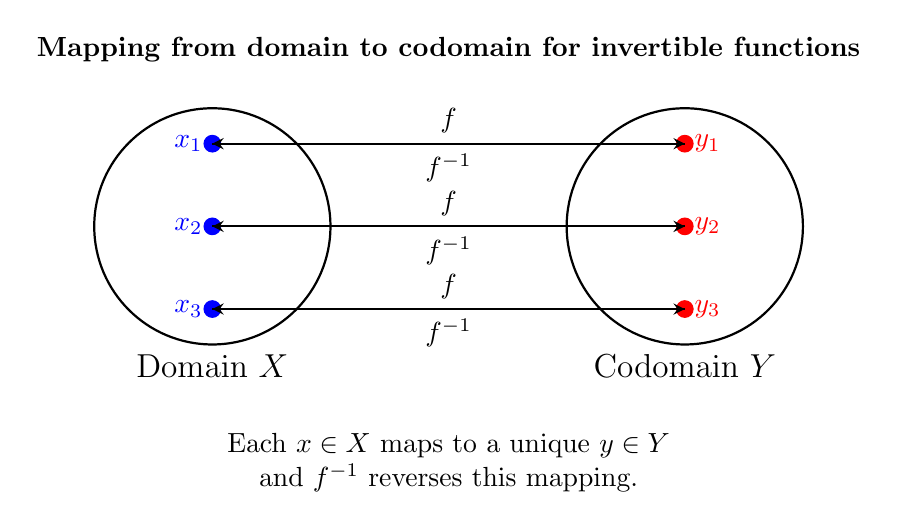
\begin{tikzpicture}[scale=1.5,>=stealth]

% Draw sets
\draw[thick] (0,0) circle(1) node[below=1.5cm] {\large Domain \(X\)};
\draw[thick] (4,0) circle(1) node[below=1.5cm] {\large Codomain \(Y\)};

% Draw points in X
\filldraw[blue] (0,0.7) circle(2pt) node[left] {\(x_1\)};
\filldraw[blue] (0,0) circle(2pt) node[left] {\(x_2\)};
\filldraw[blue] (0,-0.7) circle(2pt) node[left] {\(x_3\)};

% Draw points in Y
\filldraw[red] (4,0.7) circle(2pt) node[right] {\(y_1\)};
\filldraw[red] (4,0) circle(2pt) node[right] {\(y_2\)};
\filldraw[red] (4,-0.7) circle(2pt) node[right] {\(y_3\)};

% Draw mappings for f
\draw[->, thick] (0,0.7) -- (4,0.7) node[midway, above] {\(f\)};
\draw[->, thick] (0,0) -- (4,0) node[midway, above] {\(f\)};
\draw[->, thick] (0,-0.7) -- (4,-0.7) node[midway, above] {\(f\)};

% Draw mappings for f^{-1}
\draw[->, thick, dashed] (4,0.7) -- (0,0.7) node[midway, below] {\(f^{-1}\)};
\draw[->, thick, dashed] (4,0) -- (0,0) node[midway, below] {\(f^{-1}\)};
\draw[->, thick, dashed] (4,-0.7) -- (0,-0.7) node[midway, below] {\(f^{-1}\)};

% Annotation for invertibility
\node[align=center] at (2, 1.5) {\textbf{Mapping from domain to codomain for invertible functions}};
\node[align=center] at (2, -2) {Each \(x \in X\) maps to a unique \(y \in Y\)\\ and \(f^{-1}\) reverses this mapping.};

\end{tikzpicture}

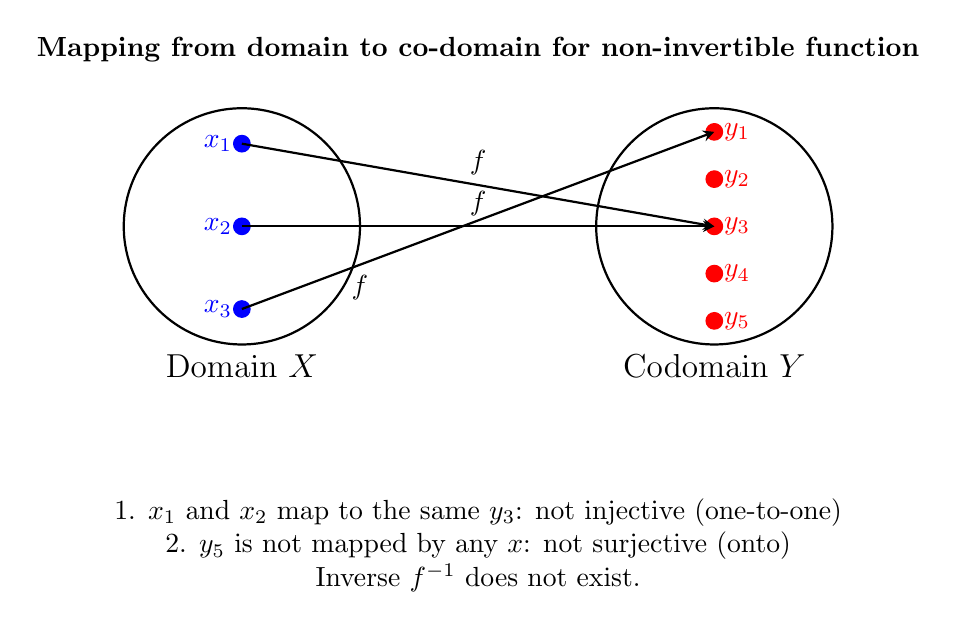
\begin{tikzpicture}[scale=1.5,>=stealth]

% Draw sets
\draw[thick] (0,0) circle(1) node[below=1.5cm] {\large Domain \(X\)};
\draw[thick] (4,0) circle(1) node[below=1.5cm] {\large Codomain \(Y\)};

% Draw points in X
\filldraw[blue] (0,0.7) circle(2pt) node[left] {\(x_1\)};
\filldraw[blue] (0,0) circle(2pt) node[left] {\(x_2\)};
\filldraw[blue] (0,-0.7) circle(2pt) node[left] {\(x_3\)};

% Draw points in Y
\filldraw[red] (4,0.8) circle(2pt) node[right] {\(y_1\)};
\filldraw[red] (4,0.4) circle(2pt) node[right] {\(y_2\)};
\filldraw[red] (4,0) circle(2pt) node[right] {\(y_3\)};
\filldraw[red] (4,-0.4) circle(2pt) node[right] {\(y_4\)};
\filldraw[red] (4,-0.8) circle(2pt) node[right] {\(y_5\)};

% Draw mappings for f
\draw[->, thick] (0,0.7) -- (4,0) node[midway, above] {\(f\)};
\draw[->, thick] (0,0) -- (4,0) node[midway, above] {\(f\)};
\draw[->, thick] (0,-0.7) -- (4,0.8) node[near start, below] {\(f\)};



% Annotation for non-invertibility
\node[align=center] at (2, 1.5) {\textbf{Mapping from domain to co-domain for non-invertible function}};
\node[align=center] at (2, -2.7) {
1. \(x_1\) and \(x_2\) map to the same \(y_3\): not injective (one-to-one)\\
2. \(y_5\) is not mapped by any \(x\): not surjective (onto)\\
Inverse \(f^{-1}\) does not exist. 
};

\end{tikzpicture}

\subsection{Proof: Inverse functions are linear}
\textbf{Property:} If \( T: V \to W \) is a linear transformation with an inverse \( T^{-1}: W \to V \), then \( T^{-1} \) is also linear.

\smallskip

\textbf{Proof:}
Let \( \mathbf{w}_1, \mathbf{w}_2 \in W \) and \( c \in \mathbb{R} \). Since \( T^{-1} \) is defined as the unique transformation such that \( T(T^{-1}(\mathbf{w})) = \mathbf{w} \), we need to show:
\[
T^{-1}(c \mathbf{w}_1 + \mathbf{w}_2) = c T^{-1}(\mathbf{w}_1) + T^{-1}(\mathbf{w}_2).
\]

Let \( \mathbf{v}_1 = T^{-1}(\mathbf{w}_1) \) and \( \mathbf{v}_2 = T^{-1}(\mathbf{w}_2) \), so \( T(\mathbf{v}_1) = \mathbf{w}_1 \) and \( T(\mathbf{v}_2) = \mathbf{w}_2 \). Then:
\[
T^{-1}(c \mathbf{w}_1 + \mathbf{w}_2) = T^{-1}(T(c \mathbf{v}_1 + \mathbf{v}_2)).
\]
Since \( T^{-1}(T(\mathbf{v})) = \mathbf{v} \), this simplifies to:
\[
T^{-1}(c \mathbf{w}_1 + \mathbf{w}_2) = c \mathbf{v}_1 + \mathbf{v}_2 = c T^{-1}(\mathbf{w}_1) + T^{-1}(\mathbf{w}_2).
\]
Thus, \( T^{-1} \) is linear.

\subsection{Proof: Invertibility implies a unique solution to $f(x)=y$}

\textbf{Property:} For a transformation (or function) $f: X \to Y$  for which there exists $f ^{-1}: Y \to X$ such that $f^{-1} \circ f = I_x$. The function is invertible, there exists for every $y \in Y$  a unique solution $x \in X$ such that $f(x)=y$. 


\textbf{Proof:} Given that $f$ is invertible, applying the inverse function on $f(x)=y$ for any $y$ gives: 

$$f^{-1}(f(x)) = f^{-1}(y)$$

which by the definition is equivalent to:

$$I_x(x) = (f^{-1} \circ f)(x) = x = f^{-1}(f(x)) = f^{-1}(y)$$

$$x = f^{-1}(y)$$

Hence, proved. Since $f$ is invertible there is only one inverse function and therefore $x$ must be unique. 

\begin{center}

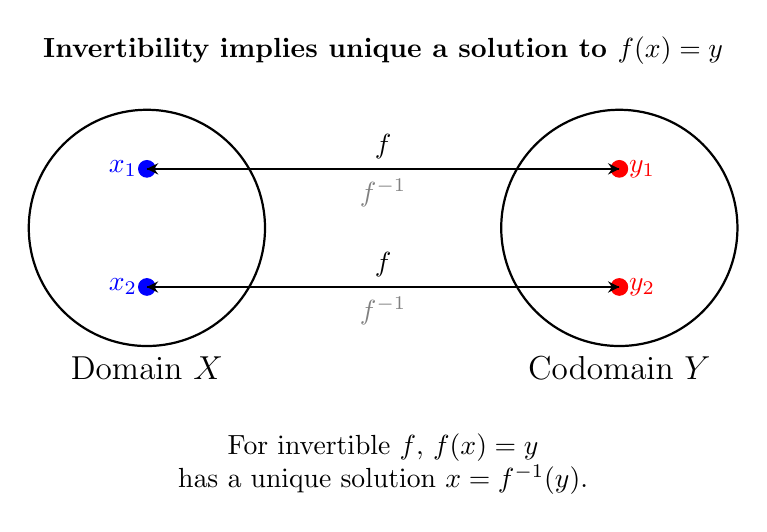
\begin{tikzpicture}[scale=1.5,>=stealth]

% Draw sets
\draw[thick] (0,0) circle(1) node[below=1.5cm] {\large Domain \(X\)};
\draw[thick] (4,0) circle(1) node[below=1.5cm] {\large Codomain \(Y\)};

% Draw points
\filldraw[blue] (0,0.5) circle(2pt) node[left] {\(x_1\)};
\filldraw[blue] (0,-0.5) circle(2pt) node[left] {\(x_2\)};
\filldraw[red] (4,0.5) circle(2pt) node[right] {\(y_1\)};
\filldraw[red] (4,-0.5) circle(2pt) node[right] {\(y_2\)};

% Draw mappings
\draw[->, thick] (0,0.5) -- (4,0.5) node[midway, above] {\(f\)};
\draw[->, thick] (4,0.5) -- (0,0.5) node[midway, below] {\color{gray} \(f^{-1}\)};

\draw[->, thick] (0,-0.5) -- (4,-0.5) node[midway, above] {\(f\)};
\draw[->, thick] (4,-0.5) -- (0,-0.5) node[midway, below] {\color{gray} \(f^{-1}\)};

% Annotations
\node at (2, 1.5) {\textbf{Invertibility implies unique a solution to $f(x)=y$}};
\node[align=center] at (2, -2) {For invertible \(f\), \(f(x) = y\)\\ has a unique solution \(x = f^{-1}(y)\).};

\end{tikzpicture}

\end{center}

\subsection{Proof: Unique solution to $f(x)=y$ implies invertibility}

This proof follows directly from the previous proof, and is essentially equivalent. 

\smallskip

\textbf{Property:} For a function $f: X \to Y$, for every $y \in Y$  for which there exists a unique solution to $f(x)=y$. The function is invertible, meaning: $f^{-1}: Y \to X$ such that $f^{-1} \circ f = I_x$. 

\smallskip

\textbf{Proof:} Given that there exists a unique solution to $f(x)=y$. 

\smallskip 
The composition of the function $f$ with the inverse function  $f^{-1}$ gives:

$$(f\circ f^{-1})(y) = y$$

which is equivalent to: 

$$I_{y}(y)= y = f\circ f^{-1} = I_{y}$$

The composition of the inverse function $f^{-1}$ with the function $f$ gives:

$$(f^{-1} \circ f)(x) = x$$

which by the definition is equivalent to:

$$I_x(x) = (f^{-1} \circ f)(x) = x = f^{-1}(f(x)) = f^{-1}(y)$$

$$x = f^{-1}(y)$$

The function $f$ satisfies the conditions of invertbility since there exists an inverse function $f^{-1}: Y \to X$ such that the composition of $f^{-1} \circ f = I_x$ and $f \circ f^{-1} = I_y$. There exists only one inverse function and hence proved that $f$ must be invertible if there exists a unique solution to $f(x) = y$ .

\subsection{Conditions for invertibility}

A function $f: \mathbb{R}^n \to \mathbb{R}^m$, where $f(\vec{x}) = \underset{m \times n}{A} \vec{x}$ is invertible \textbf{if and only if} it is bijective, that is if it satisfies two conditions: 

\begin{itemize}

\item (1) The function is surjective, that is: there exists at least one element $x$ in the domain $\mathbb{R}^n$ such that $f(x) = y$, where $y \in \mathbb{R}^m$. 

	\begin{itemize}
	
	\item If a function $f$ is surjective, the \textbf{rank(A) = m} 	
	
	\end{itemize}

\item (2) The function is injective, that is: there exist at most one element $x$ in the domain $\mathbb{R}^n$ such that $f(x) = y$, where $y \in \mathbb{R}^m$. That is, if $f(x_1) = f(x_2) \Leftrightarrow x_1 = x_2$

	\begin{itemize}
	
	\item If a function $f$ is injective, the \textbf{rank(A) = n} 	
	
	\end{itemize}


Notice that two conditions must be fulfilled for a function/linear transformation to be invertible: rank(A) = m and rank(A) = n. This implies that $m=n$, which means that the matrix $A$ must be a square matrix. Additionally, $A$ is square matrix where every column vector is linearly independent. That is: 

$$\underset{n \times n}{A} = \begin{bmatrix}

\vec{a_1} & \vec{a_2} &. &. &. &. &\vec{a_n} 


\end{bmatrix}$$

The reduced-row echelon form of $A$: 

$$rref(A) = \begin{bmatrix}


1 & 0 &. &. &. &. &0 \\
0 & 1 &. &. &. &. &0 \\
1 & 0 &. &. &. &. &0 \\
. &. &. &. &. &.  &. \\
. &. &. &. &. &. &. \\
. &. &. &. &. &. &. \\
. &. &. &. &. &. &1

\end{bmatrix} = I_n$$

Notice that the reduced-row echelon form of $A$ is just the identity matrix for $\mathbb{R}^n$.
\end{itemize}

A square matrix \( A \) is invertible if and only if the following conditions hold:
\begin{enumerate}
    \item \( \det(A) \neq 0 \).
    \item \( A \) is of full rank (i.e., rank\( (A) = n \), where \( n \) is the size of \( A \)).
    \item The rows (or columns) of \( A \) are linearly independent.
\end{enumerate}

\subsection{Method for finding inverses}
The inverse of a square matrix \( \underset{n \times n}{A} \) can be computed using the following methods:


Performing Gaussiam elimination to a matrix $A$ to get it into reduced-row echelon form is equivalent to performing linear transformations. 
\smallskip

\textbf{Further explanation:} Let $A$ be a square matrix, and the transformations $S_1, S_2 ... S_n$ be the elemenatry operations which the matrix in reduced-row echelon. It is known that: $A^{-1}A = I_n$, then the transformations: $S_1, S_2 ... S_n$ must be equal to $A^{-1}$.

\bigskip

Follow these steps to calculate the the inverse matrix $A^{-1}$ :

\begin{enumerate}

\item Form the augmented matrix of $A$ with the identity matrix $I$: 


$$\begin{bmatrix}

A | I

\end{bmatrix}$$

\item Apply row reduction to transform the matrix into the identity matrix $I$. The resulting matrix \( [I | A^{-1}] \) contains \( A^{-1} \) on the right. That is:

$$\begin{bmatrix}


I | A^{-1}

\end{bmatrix}$$

\end{enumerate}

\subsubsection{Examples:}

\paragraph{Problem:}

Let $A = \begin{bmatrix}

1 & -1 & -1 \\
1 & 2 & 3  \\
1 & -1 & 4


\end{bmatrix}$ Find the inverse matrix $A^{-1}$.

\smallskip

\textbf{Solution:} Form a matrix $B$, which is the matrix $A$ augmented with the identity matrix. $ B = \begin{bmatrix}

1 & -1 & -1 &| &1 & 0 & 0 \\
1 & 2 & 3   &| &0 & 1 & 0 \\
1 & -1 & 4  &| &0 & 0 & 1 

\end{bmatrix}$

Perform elementary row operations to get the matrix into reduced-row echelon form. 

$$ \begin{bmatrix}

1 & -1 & -1 &| &1 & 0 & 0 \\
0 & 1 & 2   &| &1 & 1 & 0 \\
0 & 2 & 5  &| &-1 & 0 & 1 

\end{bmatrix}$$


$$ \begin{bmatrix}

1 & 0 & 1 &| &2 & 1 & 0 \\
0 & 1 & 2   &| &1 & 1 & 0 \\
0 & 0 & 1  &| &-3 & -2 & 1 

\end{bmatrix}$$

$$ \begin{bmatrix}

1 & 0 & 0 &| &5 & 3 & -1 \\
0 & 1 & 0   &| &7 & 5 & -2 \\
0 & 0 & 1  &| &-3 & -2 & 1 

\end{bmatrix}$$

The left side of this matrix is the inverse matrix of $A$, so $A^{-1}$. 

\subsubsection{Finding a general formula for the inverse of 2x2 matrix}

\paragraph{Problem:}

Let $A = \begin{bmatrix}

a & b \\
c & d  \\


\end{bmatrix}$ Find the inverse matrix $A^{-1}$.


\smallskip

\textbf{Solution:} Form a matrix $B$, which is the matrix $A$ augmented with the identity matrix. $$ B = \begin{bmatrix}

a & b & | &1 & 0 \\
c & d & | &0 & 1\\

\end{bmatrix}$$


Perform elementary row operations to get the matrix into reduced-row echelon form. The transformation which corresponds to the first reduced-row operation is: $T(\begin{bmatrix}
x_1 \\ x_2 \end{bmatrix}) = \begin{bmatrix}

x_1 \\
ax_2 - cx_1

\end{bmatrix}$. Applying this transformation on our matrix results in: 

$$T(B) = \begin{bmatrix}

a & b &|& 1 & 0 \\
0 & ad-bc &|&-c & a

\end{bmatrix}$$

Continue by performing elementary row operations. The transformation which corresponds to the second reduced-row operation is: $T(\begin{bmatrix}
x_1 \\ x_2 \end{bmatrix}) = \begin{bmatrix}


(ad-bc)x_1 - b(x_2) \\

x_2

\end{bmatrix}$. Applying this transformation on our matrix results in: 


$$\begin{bmatrix}


a(ad-bc) & 0 & | & ad & -ab\\
0 & ad-bc & | &  -c & a

\end{bmatrix}$$

Continuing this process: $T(\begin{bmatrix}
x_1 \\ x_2 \end{bmatrix}) = \begin{bmatrix}


\frac{x_1}{a(ad-bc)} \\

\frac{x_2}{ad-bc}

\end{bmatrix}$. Applying this transformation on our matrix results in: 


$$T(\begin{bmatrix}
x_1 \\ x_2 \end{bmatrix}) = \begin{bmatrix}


1 & 0 & | & \frac{d}{(ad-bc)} &  \frac{-b}{(ad-bc)} \\
0 & 1 & | &  \frac{-c}{(ad-bc)} &  \frac{a}{(ad-bc)} 

\end{bmatrix}$$. 

The right part of the augmented matrix represents the inverse of our matrix $A$. Since, we solved the generalized form of the problem the solution is a general formula for finding the inverse for a 2x2 matrix. That is, for any 2x2 matrix; it's inverse will be given by the formula: 


$$ A^{-1} = \begin{bmatrix}

\frac{d}{(ad-bc)} &  \frac{-b}{(ad-bc)} \\
\frac{-c}{(ad-bc)} &  \frac{a}{(ad-bc)} 

\end{bmatrix} \qquad \text{or} \qquad A^{-1} =  \frac{1}{ad-bc} \begin{bmatrix}

d & -b \\
-c &  a


\end{bmatrix}
$$

Observe that the matrix \textbf{does not} have an inverse or rather the inverse is not defined if the terms $ad-bc=0$. That is, if $ad-bc \neq 0 \Leftrightarrow \text{A is invertible}$. The value of $ad-bc$ is important and even has a special name: it is called the \textbf{determinant}, often abbreviated as $\det()$.

\section{Determinants}

\subsection{Definition of a determinant}
The determinant is a scalar value \textbf{only defined for square matrices} which provides information about the properties about the matrix. 


\subsubsection{Connection with invertibility of a matrix}

The determinant represents useful information about the invertibility of a matrix. A matrix is invertible \textbf{if and only if} the determinant is not zero. 

\subsection{Determinant of a 2x2 matrix}

For a \( 2 \times 2 \) matrix:
\[
\underset{2x2}{A} = \begin{bmatrix}
a & b \\
c & d
\end{bmatrix},
\]
the determinant is defined as:
\[
\det(A) = ad - bc.
\]


\subsection{Determinant of a 3x3 matrix \label{Determinant of a 3x3 matrix}}


For a \( 3 \times 3 \) matrix:
\[
\underset{3x3}{A} = \begin{bmatrix}
a_{11} & a_{12} & a_{13} \\
a_{21} & a_{22} & a_{23} \\
a_{31} & a_{32} & a_{33}
\end{bmatrix},
\]
the determinant is defined as:
\[
\det(A) = a_{11} \cdot \det(\begin{bmatrix}
a_{22} & a_{23} \\
a_{32} & a_{33}
\end{bmatrix})  - a_{12} \cdot \det(\begin{bmatrix}
a_{21} & a_{23} \\
a_{31} & a_{33}
\end{bmatrix})  + a_{13} \cdot (\begin{bmatrix}
a_{21} & a_{22} \\
a_{31} & a_{32}.	
\end{bmatrix})
\] 
\subsection{General formula for the determinant of a $n \times n$ matrix}

For larger matrices, the determinant is defined recursively using cofactor expansion:
\[
\det(A) = \sum_{j=1}^n (-1)^{i+j} a_{ij} \det(M_{ij}),
\]
where \( M_{1j} \) is the minor matrix obtained by removing the first row and \( j \)-th column of \( A \).


\subsubsection{Geometric Interpretation}
The determinant represents:
\begin{itemize}
    \item The scaling factor of the transformation represented by \( A \).
    \item The signed (meaning: positive or negative  sign)volume of the parallelepiped spanned by the row (or column) vectors of \( A \).
\end{itemize}

\subsection{Determinants along other rows/columns.}

The determinant can be calculated along other rows/columns than the first row. This may be advantageous and less computionally heavy (and/or difficult) if the chosen row contains more zeros than other rows. This flexibility comes from the properties of determinants and the cofactor expansion formula. The determinant remains the same no matter which row or column is used for the expansion.

\subsubsection*{General formula for cofactor Expansion}
For a square matrix $A$ of size $n \times n$:

$$
\det(A) = \sum_{j=1}^{n} a_{ij}C_{ij} \quad \text{(Expansion along row $i$)},
$$
or
$$
\det(A) = \sum_{i=1}^{n} a_{ij}C_{ij} \quad \text{(Expansion along column $j$)},
$$
where:
\begin{itemize}
    \item $a_{ij}$ is the element in the $i$-th row and $j$-th column,
    \item $C_{ij}$ is the cofactor of $a_{ij}$, defined as:
    $$
    C_{ij} = (-1)^{i+j} \det(M_{ij}),
    $$
    where $M_{ij}$ is the $(n-1) \times (n-1)$ minor matrix obtained by removing the $i$-th row and $j$-th column from $A$.
\end{itemize}

\textbf{Note: } The cofactor expansion has a pattern which resembles a "chess board". That is for a $n \times n$ matrix the cofactor will switch sign as: $$\begin{bmatrix}


+ & - & + & - \\
- & + & - & + \\
+ & - & + & - \\
- & + & - & + \\

\end{bmatrix} $$

\subsubsection*{How to expand along other Rows or columns}
\begin{enumerate}
    \item \textbf{Choose a Row or Column:} You can expand along any row or column. Often, the row or column with the most zeros is chosen to simplify the calculations.
    \item \textbf{Calculate Cofactors:} For each element in the chosen row or column, calculate its cofactor.
    \item \textbf{Sum the Products:} Multiply each element by its cofactor and sum the results to get the determinant.
\end{enumerate}

\subsubsection*{Example}
Given a $3 \times 3$ matrix:
\[
A = \begin{bmatrix}
1 & 2 & 3 \\
0 & 4 & 5 \\
1 & 0 & 6
\end{bmatrix},
\]
we compute the determinant using expansion along different rows or columns.

\paragraph{Expansion along row 1:}
\[
\det(A) = 1 \cdot \det(\begin{bmatrix} 4 & 5 \\ 0 & 6 \end{bmatrix})
- 2 \cdot \det (\begin{bmatrix} 0 & 5 \\ 1 & 6 \end{bmatrix}) 
+ 3 \cdot \det(\begin{bmatrix} 0 & 4 \\ 1 & 0 \end{bmatrix})
\]

\paragraph{Expansion along column 1:}
\[
\det A = 1 \cdot \det(\begin{bmatrix} 4 & 5 \\ 0 & 6 \end{bmatrix})
- 0 \cdot \det (\begin{bmatrix} 2 & 3 \\ 0 & 6 \end{bmatrix})
+ 1 \cdot \det(\begin{bmatrix} 2 & 3 \\ 4 & 5 \end{bmatrix})
\]

The result will be the same, regardless of the row or column chosen. 


\subsubsection{Rule of Sarrus for determinants}
\textbf{Property:} Let $A$ be any 3x3 matrix. The determinant can be calculated efficiently using the rule of Sarrus.

\includegraphics[width=\textwidth]{Rule-of-Sarrus.png}



The rule of Sarrus gives: $$\det(A) = a_1 b_2 c_3 + b_1 c_2 a_3 + c_1 a_2 b_3 - c_1 b_2 a_3 - a_1 c_2 b_3 - b_1 a_2 c_3 $$

\textbf{Proof:} \textit{The following proof is similiar to the calculation of the determinant presented in \ref{Determinant of a 3x3 matrix}, but has been reiterated here for continuity and readability.}

Let $A$ be a 3x3 matrix: 

$$\underset{3x3}{A} = \begin{bmatrix}

a & b & c \\
d & e & f \\
g & h & i 

\end{bmatrix}$$

$$ \det(\underset{3x3}{A}) = a \begin{bmatrix}

e & f \\
h & i

\end{bmatrix} - b \begin{bmatrix}

d & f \\
g & i

\end{bmatrix} + c \begin{bmatrix}

d & e  \\
g & h

\end{bmatrix}$$


$$=a(ei -fh) - b(di-fg) + c(dk-eg)$$

$$= aei -afh - bdi + bfg + cdk -ceg $$

$$=aei+bfg+cdh-afk-bdi-ceg$$

The result of this calculation of the determinant according to its definition is the desired rule of Sarrus. Hence, proved.

\subsubsection{\label{Determinant of scalar multiplications of a row}Determinant of scalar multiplications of a row}

\textbf{Property: } Let $A$ be a $n \times n$ matrix, and $B$ be a matrix such that  one of it's row is a scalar multiple of a row in $A$. Then, \det($B$) $=$ $k$\det($A$). 

\textbf{Proof: } Let $A$ and $B$ be a $n \times n$ matrix such that: 

$$\underset{n \times n}{A} = \begin{bmatrix}

a_{11} & a_{12} &. &. &. &. &a_{1n}\\
.\\
.\\

\color{blue} a_{i1} & \color{blue} a_{i2} \color{blue} &\color{blue}. &\color{blue}. &\color{blue}. &\color{blue}. &\color{blue}a_{in} \normalcolor \\

.\\
.\\
.\\
a_{n1} & a_{n2} &. &. &. &. &a_{nn}


\end{bmatrix} \quad \underset{n \times n}{B}= \begin{bmatrix}

a_{11} & a_{12} &. &. &. &. &a_{1n}\\
.\\
.\\

\color{red} ka_{i1} & \color{red}ka_{i2} &\color{red}. &\color{red}. &\color{red}. &\color{red}. &\color{red}ka_{in} \normalcolor \\

.\\
.\\
.\\
a_{n1} & a_{n2} &. &. &. &. &a_{nn}


\end{bmatrix} $$


\begin{itemize}

\item Choosing to expand along the row $a_{i1} ... a_{in}$: will result in: $$\det(A) = (-1)^{i+1} a_{i1} M_{i1} + (-1)^{i+2} a_{i2} M_{i2} + ... + (-1)^{i+n} a_{in} M_{in}$$

\item This sum can be simplified using the general formula for the determinant of a matrix: \[
\det(A) = \sum_{j=1}^n (-1)^{i+j} a_{ij} \det(M_{ij})
\] 

\end{itemize}

\begin{itemize}



\item The determinant of matrix $B$ can be written in a similar manner. Choosing to expand along the row $ka_{i1} ... ka_{in}$, we get: $$\det(A) = (-1)^{i+1} ka_{i1} M_{i1} + (-1)^{i+2} ka_{i2} M_{i2} + ... + (-1)^{i+n} ka_{in} M_{in}$$

\item Using the general formula for the determinant of a $n \times n$ matrix, this sum can be written as: \[
\det(B) = \sum_{j=1}^n (-1)^{i+j} ka_{ij} \det(M_{ij})
\]

\item Factor out $k$ gives: \[
\det(B) = k \sum_{j=1}^n (-1)^{i+j} a_{ij} \det(M_{ij})
\]

\end{itemize}

Notice that the term $$\sum_{j=1}^n (-1)^{i+j} a_{ij} \det(M_{ij}) $$ is determinant of matrix $A$. That is. \det($B$) = $k$\det($A$). \bigskip 

Hence, proved that the determinant of any matrix when a single row of its is multiplied by a scalar is \textbf{scaled by the same value}.  

\subsubsection{\label{Determinant of a matrix when row is added} Determinant of a matrix when row is added}


\textbf{Property: } Let $A$, $B$, $C$ be $n \times n$ matrices. Let $A$ and $B$ such matrices which only differ in their $i$th row, and let $C$ be a matrix such that one of it's row consists of the addition of the $i$th row in $A$ and $B$. Then: \det($C$) $=$ \det($A$) $+$ \det($B$). 


\textbf{Proof: } Let $A$, $B$ and $C$ be $n \times n$ matrices such that: 

$$\underset{n \times n}{A} = \begin{bmatrix}

a_{11} & a_{12} &. &. &. &. &a_{1n}\\
.\\
.\\

\color{blue} x_{i1} & \color{blue} x_{i2} \color{blue} &\color{blue}. &\color{blue}. &\color{blue}. &\color{blue}. &\color{blue}x_{in} \normalcolor \\

.\\
.\\
.\\
a_{n1} & a_{n2} &. &. &. &. &a_{nn}


\end{bmatrix} \quad \underset{n \times n}{B}= \begin{bmatrix}

a_{11} & a_{12} &. &. &. &. &a_{1n}\\
.\\
.\\

\color{red} y_{i1} & \color{red}y_{i2} &\color{red}. &\color{red}. &\color{red}. &\color{red}. &\color{red}y_{in} \normalcolor \\

.\\
.\\
.\\
a_{n1} & a_{n2} &. &. &. &. &a_{nn}


\end{bmatrix} $$

$$\underset{n \times n}{C} = \begin{bmatrix}


a_{11} & a_{12} &. &. &. &. &a_{1n}\\
.\\
.\\

\color{blue} x_{i1} + \color{red} y_{i1} & \color{blue} x_{i2} + \color{red} y_{i2}  \color{blue} &\color{blue}. &\color{blue}. &\color{blue}. &\color{blue}. &\color{blue}x_{in} + \color{red} y_{in} \normalcolor \\

.\\
.\\
.\\
a_{n1} & a_{n2} &. &. &. &. &a_{nn}

\end{bmatrix}$$


\smallskip 
Let us look at the determinants of matrix $A$, $B$ and $C$ indiviudally if we choose to expand along the $i$th row:


\begin{enumerate}


\item Determinant of matrix $A$: 

	$$\det(A)=\sum_{j=1}^n (-1)^{i+j} x_j \det(M_{ij})$$

\item Determinant of matrix $B$: 

	$$\det(B)=\sum_{j=1}^n (-1)^{i+j} y_j \det(M_{ij})$$

\item Determinant of matrix $C$: 

	$$\det(C)=\sum_{j=1}^n (-1)^{i+j} (x_j + y_j) \det(M_{ij})$$
	
	\begin{itemize}
	
	\item Notice that the determinant is the sum of the determinants of $A$ and $B$. That is: $\det(C) = \det(A) + \det(B)$  

	\end{itemize}
	
\end{enumerate}

Hence, proved. The determinant of a matrix of which one row is a the sum of rows of two other matrices is the sum of the determinants of those matrices themselves.

\subsubsection{Determinant of matrix after row swapping}

\textbf{Property: } The determinant of a matrix changes sign when a row is swapped. For two $n \times n$ matrices $A$ and $B$. Then: $\det(B) = -\det(A)$: 

$$\underset{n \times n}{A} = \begin{bmatrix}

\vec{r_1} \\
.\\
.\\
\vec{r_i} \\
.\\
.\\
\vec{r_j} \\
.\\
.\\
\vec{r_n}

\end{bmatrix} \quad and \quad \underset{n \times n}{B} = \begin{bmatrix}

\vec{r_1} \\
.\\
.\\
\vec{r_j} \\
.\\
.\\
\vec{r_i} \\
.\\
.\\
\vec{r_n}

\end{bmatrix} $$


\textbf{Proof: } Let $A$ and $B$ matrices, as shown above. Calculate the determinant for each respective matrix by expanding along the $i$th row. 

\begin{itemize}

\item Determinant for $A$:

$$\det(A) = \sum_{j=1}^{j=n} (-1)^{i+j}a_{ij}\det(M_{ij})$$


\item After the swap, row $i$ now becomes row $j$, and row $j$ becomes row $i$. If we expand along $i$th row to calculate the determinant of $B$: 


$$\det(B) = \sum_{j=1}^{j=n} (-1)^{i+j}a_{kj}\det(M_{kj})$$

\item This flips the order of the elements, and hence changes the sign factor $(-1)^{i+j}$ which is equivalent to multiplying the row by $-1$. 


\end{itemize}

Notice that $M_{kj}$ remains the same because the minor matrix $M_{kj}$ only depends on the rows and columns not being used, and the row swap only affects the top-level row structure. The only difference is that the expansion uses elements $a_{kj}$ instead of $a_{ij}$. 

Hence, proved. The determinant of a matrix is multiplied by $-1$ if we swap two rows.


\subsubsection{\label{Determinant of a matrix with duplicate rows}Determinant of a matrix with duplicate rows}

\textbf{Property: } The determinant of a matrix with duplicate rows is zero. 

\textbf{Additional explanation: }This infers that it is not invertible. It infers that the reduced row-echelon form will not be the identity matrix.

\textbf{Proof: } Let $A$ and $B$ be two $n \times n$ matrices. Let $B$ be similar to matrix $A$ in all respects except which except two of its rows have been swapped. If row $i$ is a duplicate of row $j$, or vice-versa.  That is, if $A$ and $B$ are two matrices such that: $$\underset{n \times n}{A} = \begin{bmatrix}

\vec{r_1} \\
.\\
.\\
\vec{r_i} \\
.\\
.\\
\vec{r_j} \\
.\\
.\\
\vec{r_n}

\end{bmatrix} \quad and \quad \underset{n \times n}{B} = \begin{bmatrix}

\vec{r_1} \\
.\\
.\\
\vec{r_j} \\
.\\
.\\
\vec{r_i} \\
.\\
.\\
\vec{r_n}

\end{bmatrix}$$


\begin{center}

where the row vectors are $\vec{r_x} = [a_{1}, a_{2}, \dots , a_{n} ]$ and \textbf{$\vec{r_i} = \vec{r_j}$}.

\end{center}

\begin{itemize}

\item It is known that the determinant changes sign if two rows have been swapped. That is: $\det(B) = -\det(A)$

\item If row $i$ = row $j$, which explicitly means that the matrices are: $A=B$. This infers that $\det(B) = - \det(A)$. However since the matrices are the exact same, it must hold that: $\det(A) \Leftrightarrow \det(B)$, therefore if $\det(B) = - \det(A)$, it must mean that both $\det(A) = \det(B) = 0$ 

\end{itemize}

Hence, proved that if a matrix contains duplicate rows it's determinant is zero. 


\subsubsection{Determinant of a matrix after elementary row operations}

\textbf{Property}: For a matrix $A$, performing elementary row operations does not change the determinant. 

\textbf{Proof: } Let $A$ and $B$ be two $n \times n$ matrices. Let $B$ be similar to matrix $A$ in all respects except that one of its rows contains itself minus a scalar multiple of another row. That is: $$\underset{n \times n}{A} = \begin{bmatrix}

\vec{r_1} \\
.\\
.\\
\vec{r_i} \\
.\\
.\\
\vec{r_j} \\
.\\
.\\
\vec{r_n}

\end{bmatrix} \quad and \quad \underset{n \times n}{B} = \begin{bmatrix}

\vec{r_1} \\
.\\
.\\
\vec{r_i} \\
.\\
.\\
\vec{r_j} - c\vec{r_i}  \\
.\\
.\\
\vec{r_n}

\end{bmatrix}$$


\begin{center}

where the row vectors are $\vec{r_x} = [a_{x1}, a_{x2} ... a_{xn} ]$.

\end{center}

Let's look closely at the determinant of $B$. 

\begin{itemize}

\item Recall that (as mentioned in: \ref{Determinant of a matrix when row is added}): $$ \det(B) = \det(A) + \det \left(\begin{bmatrix}

\vec{r_1} \\
.\\
.\\
\vec{r_i} \\
.\\
.\\
- c\vec{r_i}  \\
.\\
.\\
\vec{r_n}

\end{bmatrix}\right)$$

\item Factor out $-c$, as mentioned in \ref{Determinant of scalar multiplications of a row}: 

$$\det(B) = \det(A) - cdet \left(\begin{bmatrix}

\vec{r_1} \\
.\\
.\\
\vec{r_i} \\
.\\
.\\
\vec{r_i}  \\
.\\
.\\
\vec{r_n}

\end{bmatrix}\right)$$

\item Notice that the matrix contains duplicate rows, which as mentioned in \ref{Determinant of a matrix with duplicate rows} results in the determinant becoming zero. That is: 


$$\det(B) = \det(A)$$


\end{itemize}

\paragraph{Example: } Let $\underset{4x4}{A}$ be the matrix: $$\begin{bmatrix}

1 & 2 & 2 & 1 \\
1 & 2 & 4 & 2 \\
2 & 7 & 5 & 2 \\
-1 & 4 & -6 & 3

\end{bmatrix} $$

Incomplete!!!

\subsubsection{Determinant of a 2x2 matrix and area of the paralellogram}

\textbf{Property: } Let $A$ be a 2x2 matrix, given by the column vectors $\vec{v_1}$ and $\vec{v_2}$, such that: 

$$\underset{2x2}{A} = \begin{bmatrix}


a & b \\
c & d
\end{bmatrix} \quad , where: \vec{v_1} = \begin{bmatrix}

a \\
c


\end{bmatrix} , \vec{v_2} = \begin{bmatrix}


b \\ 
d

\end{bmatrix}  $$

The area of the parallelogram spanned by $\vec{v_1}$ and $\vec{v_2}$ is equal to the determinant of $A$, that is: $ad-cb$

\textbf{Proof: } Let the area of the paralellogram be: 


\begin{center}
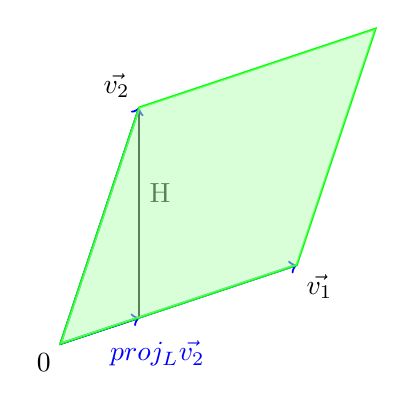
\begin{tikzpicture}
  % Define points for the parallelogram
  \coordinate (O) at (0,0); % Origin
  \coordinate (A) at (3,1); % First vector
  \coordinate (B) at (1,3); % Second vector
  \coordinate (C) at ($(A)+(B)$); % Sum of vectors

	% Add normal to \mathbf{a} at a point on \mathbf{b}
	\coordinate (P) at ($(O)!1!(B)$); % Midpoint on vector b
	\coordinate (N) at ($(P)+(0,-2.67)$); % Perpendicular vector direction (scaled)

	% Draw the normal line
	\draw[thick,black] (P) -- (N) node[midway, above right] {H};
	
	\draw[thick, blue, ->] (O) -- (N) node[midway, below right] {$proj_{L}\vec{v_2}$};

  % Draw vectors
  \draw[thick,->,blue] (O) -- (A);
  \draw[thick,->,blue] (O) -- (B);

  % Draw parallelogram
  \draw[thick,green] (O) -- (A) -- (C) -- (B) -- cycle;

  % Fill the parallelogram with semi-transparent color
  \fill[green!30,opacity=0.5] (O) -- (A) -- (C) -- (B) -- cycle;

  % Label the origin and vertices
  \node[below left] at (O) {$0$};
  \node[below right] at (A) {$\vec{v_1}$};
  \node[above left] at (B) {$\vec{v_2}$};

\end{tikzpicture}
\end{center}

\begin{itemize}

\item The base (B) is given by the length of the vector $\vec{v_1}$: $|| \vec{v_1} ||$
\item The area of a parellelogram is given by the formula: $A=B \cdot H$. 

	\begin{itemize}
	
		\item Using the Pythagorean theorem to set up the equations: $$H^2 + proj_{L}\vec{v_2}^2 = ||\vec{v_2} || ^2$$
		
		\item Move isolate $H$: $$H^2 = ||\vec{v_2} || ^2 - proj_{L}\vec{v_2}^2 $$
		
		\item Simplify the expression: $$\vec{v_2} \cdot \vec{v_2} - ||proj_{L}\vec{v_2}||^2$$
		
		\item Calculate $proj_{L}\vec{v_2}$: 
		
		$$\vec{v_2} \cdot \vec{v_2} - \frac{\vec{v_2} \cdot \vec{v_1}}{\vec{v_1} \cdot \vec{v_1}}\vec{v_1} \cdot \frac{\vec{v_2} \cdot \vec{v_1}}{\vec{v_1} \cdot \vec{v_1}}\vec{v_1} $$
		
		\item The terms $ \vec{v_1} \cdot \vec{v_1}$ cancel, yielding: 
		
		$$H^2 = \vec{v_2} \cdot \vec{v_2} - \frac{(\vec{v_2} \cdot \vec{v_1})^2}{\vec{v_1} \cdot \vec{v_1}}$$
	
	\end{itemize}


\item The area of the paralellogram squared is: $A^2=B^2 \cdot H^2$, that gives: 

	\begin{itemize}
	
		\item $B^2 = || \vec{v_1}|| ^2 = \vec{v_1} \cdot \vec{v_1}$ 
		\item $H^2 = \vec{v_2} \cdot \vec{v_2} - \frac{(\vec{v_2} \cdot \vec{v_1})^2}{\vec{v_1} \cdot \vec{v_1}} $
	\end{itemize}
\item Calculate $A^2$: 

$$A^2 = || \vec{v_1}|| ^2 = \vec{v_1} \cdot \vec{v_1} \cdot (H^2 = \vec{v_2} \cdot \vec{v_2} - \frac{(\vec{v_2} \cdot \vec{v_1})^2}{\vec{v_1} \cdot \vec{v_1}} ) $$

$$A^2 = (a^2 + b^2)(b^2 + d^2) - (ab+cd)^2$$

Simplify: 

$$A^2 = a^2b^2 + a^2d^2 + c^2d^2 - a^2b^2	 - 2abcd - c^2d^2$$

Substitute using : $x=ad$ and $y=cb$

$$A^2 = x^2 - 2xy + y^2 = (x-y)^2$$

$$A^2 = (ad-bc)^2$$

$$A = |ad-bc|$$


\end{itemize}

The determinant of a 2x2 matrix gives the area spanned by the column vectors of a paralellogram. Hence, proved. 

\subsubsection{Determinant as a scaling factor}

\textbf{Property:} For a transformation $T: \mathbb{R}^2 \to\mathbb{R}^2$ where $T(x) = Ax$, the scaling factor for the area associated with two vectors is $\det(A)$. 


\textbf{Proof:} Consider a $2 \times 2$ matrix $A$ given by:
\[
A = \begin{bmatrix} a & b \\ c & d \end{bmatrix}.
\]
Let the following be position vectors, which when connected form a rectangle: $$\vec{a} = \begin{bmatrix} 0 \\ 0 \end{bmatrix}, \quad \vec{b} = \begin{bmatrix} k_1 \\ 0 \end{bmatrix},  \quad \vec{c} = \begin{bmatrix} k_1 \\ k_2 \end{bmatrix}, \quad \vec{d} = \begin{bmatrix} 0 \\ k_2 \end{bmatrix}$$

\begin{figure}[H]
\begin{center}
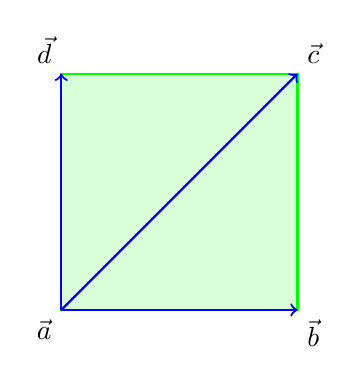
\begin{tikzpicture}
  % Define points for the parallelogram
  \coordinate (O) at (0,0); % Origin
  \coordinate (A) at (3,0); % First vector
  \coordinate (B) at (0,3); % Second vector
  \coordinate (C) at ($(A)+(B)$); % Sum of vectors

	% Add normal to \mathbf{a} at a point on \mathbf{b}
	\coordinate (P) at ($(O)!1!(B)$); % Midpoint on vector b
	\coordinate (N) at ($(P)+(0,-2.67)$); % Perpendicular vector direction (scaled)
	
	% Fill the parallelogram with semi-transparent color
	\fill[green!30,opacity=0.5] (O) -- (A) -- (C) -- (B) -- cycle;
		  % Draw parallelogram
	  \draw[thick,green] (O) -- (A) -- (C) -- (B) -- cycle;

	  % Draw vectors
	  \draw[thick,->,blue] (O) -- (A);
	  \draw[thick,->,blue] (O) -- (B);
	  \draw[thick,->,blue] (O) -- (C);
	
	
	
	  % Label the origin and vertices
	  \node[below left] at (O) {$\vec{a}$};
	  \node[below right] at (A) {$\vec{b}$};
	  \node[above left] at (B) {$\vec{d}$};
	  \node[above right] at (C) {$\vec{c}$};

\end{tikzpicture}
\end{center}
\caption{Illustration of the image of the rectangle.}
\end{figure}


Let $T$ be a linear transformation: $$T(\vec{x}) = A\vec{x}$$ 

Apply to each of the vectors: $$T(\vec{a}) = \begin{bmatrix}
0 \\ 0
\end{bmatrix}  , \quad T(\vec{b}) = \begin{bmatrix}
ak_1 \\ ck_1
\end{bmatrix} , \quad T(\vec{c}) = \begin{bmatrix}
ak_1+bk_2 \\ ck_1+dk_2
\end{bmatrix} , \quad T(\vec{d}) = \begin{bmatrix}
bk_2 \\ dk_2
\end{bmatrix}$$


Let these transformed vectors form the sides of a parallelogram in 2D. 

\begin{figure}[H]
\begin{center}
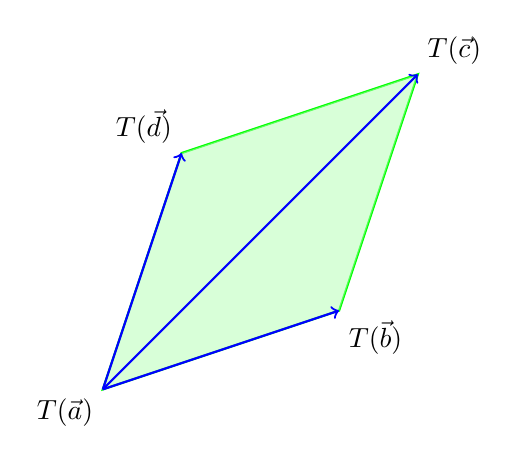
\begin{tikzpicture}
  % Define points for the parallelogram
  \coordinate (O) at (0,0); % Origin
  \coordinate (A) at (3,1); % First vector
  \coordinate (B) at (1,3); % Second vector
  \coordinate (C) at ($(A)+(B)$); % Sum of vectors

	% Add normal to \mathbf{a} at a point on \mathbf{b}
	\coordinate (P) at ($(O)!1!(B)$); % Midpoint on vector b
	\coordinate (N) at ($(P)+(0,-2.67)$); % Perpendicular vector direction (scaled)
  
  % Draw parallelogram
  \draw[thick,green] (O) -- (A) -- (C) -- (B) -- cycle;

  % Fill the parallelogram with semi-transparent color
  \fill[green!30,opacity=0.5] (O) -- (A) -- (C) -- (B) -- cycle;

  % Draw vectors
  \draw[thick,->,blue] (O) -- (A);
  \draw[thick,->,blue] (O) -- (B);
  \draw[thick,->,blue] (O) -- (C);



  % Label the origin and vertices
  \node[below left] at (O) {$T(\vec{a})$};
  \node[below right] at (A) {$T(\vec{b})$};
  \node[above left] at (B) {$T(\vec{d})$};
  \node[above right] at (C) {$T(\vec{c})$};

\end{tikzpicture}
\end{center}
\caption{Illustration of the image of the rectangle under transformation.}
\end{figure}

The area of this parallelogram is the absolute value of the determinant of a new matrix $I$ containing the column vectors: $T(\vec{d})$ and $T(\vec{b})$. 

$$\text{Area}  = I = \begin{bmatrix}

ak_1 & bk_2 \\
ck_1 & dk_2

\end{bmatrix} $$

$$|\det(I)| = |k_1k_2ad-k_1k_2bc|$$

Factor out $k_1$ and $k_2$: 

$$|\det(I)| = |k_1k_2(ad-bc)|$$

Notice that the terms: $ad-bc$ is the determinant of the transformation matrix $A$. This equation can be rewritten as: $$\text{Area} = |\det(I)| = |k_1k_2det(A)|$$

Hence, proved. The determinant of a square matrix represents the scaling factor by which the transformation associated with the matrix scales areas (in 2D) or volumes (in higher dimensions). \textbf{In clearer words:} the area under transformation bounded by any vectors in $\mathbb{R}^2$ can be written as the determinant of the transformation matrix times the area originally bounded by the vectors. 


\section{Transpose of a matrix}


\subsection{Definition of the transpose of a matrix}

Let $A$ be any nxm matrix: 
$$\underset{nxm}{A} = \begin{bmatrix}

a_{11} & a_{12} &. &. &. &. &a_{1n}\\
.\\
.\\

a_{i1} & a_{i2} &.  &. &. &. &a_{in}  \\

.\\
.\\
.\\
a_{m1} & a_{n2} &. &. &. &. &a_{mn}



\end{bmatrix}$$ 

The transpose, often denoted as $A^T$, is defined as: 

$$ \underset{m \times n}{A^T} = \begin{bmatrix}

a_{11} & a_{12} &. &. &. &. &a_{1m}\\
.\\
.\\

a_{i1} & a_{i2} &.  &. &. &. &a_{im}  \\

.\\
.\\
.\\
a_{n1} & a_{n2} &. &. &. &. &a_{nm}


\end{bmatrix}
$$

\subsection{Determinant of transpose}

\textbf{Property:} The determinant of transpose is equal to the determinant of the original matrix. $\det(A) = \det(A^{T})$. The determinant of a matrix is invariant under transposition. 

\textbf{Proof by induction:} 

\begin{enumerate}

\item The determinant for a $2 \times 2$ matrix:
\[
A = \begin{bmatrix} a & b \\ c & d \end{bmatrix}, \quad A^{T} = \begin{bmatrix} a & c \\ b & d \end{bmatrix}.
\]

The determinant of $A$ is given by:
\[
\det(A) = ad - bc.
\]

The determinant of $A^{T}$ is:
\[
\det(A^{T}) = ad - bc.
\]

\[
\det(A) = \det(A^{T}).
\]

Since both determinants are equal, conclude that the property holds for a 2x2 matrix.

\item Assume that the property holds for any $n \times n$ matrix.

\item Does the property holds for any (n+1)x(n+1) matrix?

	\begin{itemize}
	
		\item Let $A$ and $A^T$ be: $$ \underset{m \times n}{A^T} = \begin{bmatrix}

				a_{11} & a_{12} &. &. &. &. &a_{1m}\\
				.\\
				.\\
				
				a_{i1} & a_{i2} &.  &. &. &. &a_{im}  \\
				
				.\\
				.\\
				.\\
				a_{n1} & a_{n2} &. &. &. &. &a_{nm}
				
				
				\end{bmatrix} \quad \underset{nxm}{A} = \begin{bmatrix}

						a_{11} & a_{12} &. &. &. &. &a_{1n}\\
						.\\
						.\\
						
						a_{i1} & a_{i2} &.  &. &. &. &a_{in}  \\
						
						.\\
						.\\
						.\\
						a_{m1} & a_{n2} &. &. &. &. &a_{mn}
						
						
						
					\end{bmatrix}
				$$	
		\item The determinant of $\underset{nxm}{A}$ using cofactor expansion along the first row is:
			$$\det(A) = a_{11}\det(A_{11}) - a_{12}\det(A_{12}) + ... + (-1)^{1+m} \det(A_{1m})$$
		
		\item The determinant of $\underset{m \times n}{A^T}$ using cofactor expansion along the first column is:
		$$\det(A^T) = a_{11}\det(A_{11}^T) - a_{12}\det(A_{12}^T) + ... + (-1)^{1+m} \det(A_{1m}^T)$$
	
		\begin{itemize}
		
			\item The transpose of the minor matrices is equal to the original minor matrices. 
			
			\item That is: $A_{11}^T, A_{12}^T ... A_{1m}^T  = A_{11}, A_{12} ... A_{1m}$ 
			
			\item The determinant of the minor matrices is unchanged between $A$ and $A^T$. 
			\item This property holds for matrices of any size because transposition does not affect the cofactor expansion used to compute determinants.
		\end{itemize}			
		\item The determinant of $\underset{m \times n}{A^T}$ can hence be rewritten as $$\det(A^T) = a_{11}\det(A_{11}) - a_{12}\det(A_{12}) + ... + (-1)^{1+m} \det(A_{1m})$$
		
		\item The determinant of $\underset{m \times n}{A^T}$ is equal to the determinant of $\underset{nxm}{A}$. 
		$$\det(A^T) = \det(A)$$
	\end{itemize}

\end{enumerate}

Since this property holds for any matrix of size $(n+1) \times (n+1)$, it must also hold for any matrix of size $n \times n$. Hence, proved. 

\subsubsection{Transpose of a matrix product}

Let $C = AB$, and $D = B^T A^T$, then it holds that: $C^T = D = (AB)^T = B^TA^T$

\subsubsection{Transposes of sums and inverses}

Let $C=A+B$ such that: $c_{ij} = a_{ij} + b_{ij}$, then it holds that: $C^T = (A+B)^T = A^T + B^T$

\subsubsection{Transposes of a inverse}
Let $A^-1$ be the inverse of $A$, such that: $A^{-1}A = I_n$ and $AA^{-1} = I_n$. Transposing both sides: $(A^{-1}A)^{-1} = I_n^T$ and $(AA^{-1})^{-1} = I_n^T$. The transpose of the inverse is equal to the the inverse itself, and the transpose of a matrix product is equal to the product of the inverses in reverse order, that is: $(A^{-1})^T A^T = I_n$ and $A^T (A^{-1})^T  = I_n$, so $(A^{-1})^T$ is the inverse of $A^T$, meaning: $(A^T)^{-1} = (A^{-1})^{T}$

\subsubsection{Transpose of a vector}

Let $\vec{v}$ and $\vec{w}$ be two nx1 vectors, then it holds that:  $\vec{v} \cdot \vec{w} = \vec{v}^T \vec{w}$. 


Let $A$ be an $m \times n$ matrix, $\vec{x}$ be an nx1 vector and $\vec{y}$ be an mx1 vector, then it holds that: $(A\vec{x}) \cdot \vec{y} = (A\vec{x})^T \vec{y} = (\vec{x}^T A^T) \vec{y} = \vec{x}^T \cdot (A^T \vec{y}) = \vec{x}^T \cdot (A^T \vec{y})$. 


\subsubsection{Definition of the Row Space}

The row space of a matrix \(A\) is the subspace of \(\mathbb{R}^n\) spanned by its row vectors. If \(A\) is an \(m \times n\) matrix, its row space is a subspace of \(\mathbb{R}^n\). To determine the row space, one typically considers the rows of \(A\) in its row-echelon form, as the non-zero rows in this form provide a basis for the row space.

\subsubsection{Relationship Between the Null Spaces of the Row Space and the Column Space}

The null space of the row space of a matrix \(A\) corresponds to the null space of \(A^T\), the transpose of \(A\). This is because the rows of \(A\) become the columns of \(A^T\), and the null space of \(A^T\) represents all vectors orthogonal to the row space of \(A\). Similarly, the null space of \(A\) represents all vectors orthogonal to the column space of \(A\).

Key relationships include:

1. The dimension of the row space (the rank of \(A\)) and the nullity of \(A^T\) are complementary:
   \[
   \text{Rank}(A) + \text{Nullity}(A^T) = n,
   \]
   where \(n\) is the number of columns of \(A\).

2. The row space and column space are dual in the sense that transformations of \(A\) affect both spaces symmetrically.

\subsubsection{Showing that $A^T A$ is invertible}

Let $A$ be $k \times n$ matrix where all the column vectors are linearly independent. Let $B = A^T A$. $B$ will be a $k \times k$ matrix. Let $\vec{v} \in N(A^TA) \Leftarrow \vec{v}^T A^T A\vec{v} = \vec{v} \vec{0}$. Then: $(A\vec{v})^TA\vec{v} = 0  \Rightarrow A\vec{v} \cdot A\vec{v} = 0 \Rightarrow || A \vec{v} || ^2 = 0 \Leftarrow A\vec{v} = 0$.  This infers that: $N(A^T A)= N(A) = \{ \vec{0} \}$. Since, the matrix contains $k$ linearly independent vectors, it's reduced row echelon form will be the identity matrix. Let $(A^TA)\vec{x} = \vec{0}$


\section{Orthogonal complements}

\subsection{Definition of a orthogonal complement}

The orthogonal complement to $V \subseteq \mathbb{R}^n$ , often denoted as $V^T$ is defined as the set of all elements that fulfil: $$ \{ \vec{x} \in \mathbb{R} ^n | \vec{x} \cdot \vec{v} = 0; \forall \vec{v} \in V \}$$


\subsection{Null space and row space are orthogonal complements}

\textbf{Property:}  Every member of the null space of $A$ is orthogonal to the row space of $A$, or in other words: the null space of $A$ is the orthogonal complement of the row space of $A$.

\textbf{Proof:} Let $A$ be a $m \times n$ matrix. Let $\vec{v}  \in  N(A)$ and $\vec{w}  \in  C(A^T)$, then: $\vec{v} \cdot \vec{w} = 0$. The reverse is also true. Every member of the orthogonal complement to the row space of $A$ is orthogonal to the null space.

\subsection{Representing vectors in $\mathbb{R}^n$ using members of a subspace $V$ and the orthogonal complement of $V$}

\textbf{Property:}
Any vector in $\mathbb{R}^n$ can be uniquely represented as the sum of a vector in the subspace $V$ and a vector in the orthogonal complement of $V$, denoted $V^\perp$.

\textbf{Proof:}
Let $V$ and $V^\perp$ be subspaces of $\mathbb{R}^n$. We know the following facts:

- The sum of the dimensions of $V$ and $V^\perp$ is $n$, i.e.,
$ dim(V) + \dim(V^\perp) = n$ 
- Let $\dim(V) = k$, and thus $\dim(V^\perp) = n - k$.

- Let $\{ \vec{v_1}, \vec{v_2}, \dots, \vec{v_k} \}$ be a basis for $V$, and $\{ \vec{w_1}, \vec{w_2}, \dots, \vec{w_{n-k}} \}$ be a basis for $V^\perp$

Since these sets form bases for $V$ and $V^\perp$, they are linearly independent and span $V$ and $V^\perp$, respectively. Therefore, the union of these two sets:
$$ \{ \vec{v_1}, \vec{v_2}, \dots, \vec{v_k}, \vec{w_1}, \vec{w_2}, \dots, \vec{w_{n-k}} \}$$ is a set of $n$ linearly independent vectors. Since there are $n$ linearly independent vectors, this set must span the entire space $\mathbb{R}^n$.

Thus, any vector $\vec{a} \in \mathbb{R}^n$ can be written as a linear combination of these $n$ vectors. In particular, for $\vec{a} \in \mathbb{R}^n$, there exists unique scalars: $$c_1, c_2, \dots, c_k, d_1, d_2, \dots, d_{n-k}$$ such that: $$\vec{a} = \sum_{i=1}^k c_i \vec{v_i} + \sum_{j=1}^{n-k} d_j \vec{w_j}$$ This expresses $\vec{a}$ as the sum of vectors: $$\vec{v} = \sum_{i=1}^k c_i \vec{v_i} \in V \quad \vec{w} = \sum_{j=1}^{n-k} d_j \vec{w_j} \in V^\perp$$.

Now, we prove the \textbf{uniqueness} of this decomposition using proof by contradiction.

Assume that there are two different decompositions of $\vec{a}$ as:
$$\vec{a} = \vec{v_1} + \vec{w_1} = \vec{v_2} + \vec{w_2}$$ where: $$\vec{v_1}, \vec{v_2} \in V \quad \text{and} \quad \vec{w_1}, \vec{w_2} \in V^\perp$$. Subtracting these two expressions gives: $$\vec{v_1} - \vec{v_2} = \vec{w_2} - \vec{w_1}$$ Let: $$\vec{z} = \vec{v_1} - \vec{v_2} = \vec{w_2} - \vec{w_1}$$ Note that $\vec{z} \in V$ and $\vec{z} \in V^\perp$. Since the only vector that is both in a subspace and in its orthogonal complement is the zero vector, we conclude: $\vec{z} = \vec{0}$ Thus, $$\vec{v_1} = \vec{v_2} \quad \text{and} \quad \vec{w_1} = \vec{w_2}$$ This shows that the decomposition of $\vec{a}$ into a vector in $V$ and a vector in $V^\perp$ is unique. Therefore, every vector in $\mathbb{R}^n$ can be uniquely written as the sum of a vector from $V$ and a vector from $V^\perp$.



\subsubsection{The orthogonal complement of the orthogonal complement of $V$ is $V$.}
\textbf{Property:} The orthogonal complement of the orthogonal complement of $V$ is $V$. That is: $(V^{\perp})^{\perp} = V$ 

\textbf{Proof:} Let $\vec{x} \in (V^{\perp})^{\perp}$. Any vector in $\mathbb{R}^n$ can be written using a sum of a vector in $V$ and a vector in $V^{\perp}$. That is: $\vec{x} = \vec{v} + \vec{w}$ where $\vec{v} \in V$ and $\vec{w} \in V^{\perp}$. 
(1) $\vec{x} \cdot \vec{w} = 0 = (\vec{v} + \vec{w}) \cdot \vec{w} = \vec{v} \cdot \vec{w} + \vec{w} \cdot \vec{w} = || \vec{w} || ^2 \rightarrow || \vec{w} || ^2 = 0 \rightarrow  \vec{w} = \vec{0} \rightarrow \vec{x} =  \vec{v} \rightarrow  \vec{x} \in V$. That is, if $\vec{x} \in (V^{\perp})^{\perp} \rightarrow  \vec{x} \in V$. 


\subsubsection{Orthogonal complement of the null space}

\textbf{Property:} The orthogonal complement of the null space is the row space. Note that the row space is exactly equivalent to the column space of the transpose of the matrix: $Col(A^T) = Row(A)$


$N(A)^{\perp} = C(A^T)$. 

\textbf{Proof:} The row space can be written as: $(C(A^T)^{\perp} = N(A)$. Taking the orthogonal complement of both sides:  $$C(A^T)^{\perp})^{\perp} = N(A)^{\perp}$$ Since: $$(C(A^T)^{\perp})^{\perp} = C(A^T)$$ the equation can be rewritten as: $$N(A)^{\perp} = C(A^T)$$ or: 
$$Row(A)^\perp = Nul(A)$$


\subsubsection{Orthogonal complement of the left null  space}

\textbf{Property:} The orthogonal complement of the left null space is the column space of $N(A^T)^{\perp} = C(A)$. 

\textbf{Proof:} The left null space can be written as: $= N(A^T) = C(A)^{\perp} $. Taking the orthogonal complement of both sides:  $$(C(A)^{\perp})^{\perp} = N(A^T)^{\perp}$$ Since $$(C(A)^{\perp})^{\perp} = C(A)$$ the equation can be rewritten as: $$N(A^T)^\perp = C(A)$$

\subsubsection{Unique row space solution to $A\vec{x}=\vec{b}$}

\textbf{Property:} Let $A$ be a $m \times n$ matrix and $\vec{b} \in C(A)$, then: the equation $A \vec{x} = \vec{b}$ has at least one unique solution for $\vec{x} \in \mathbb{R}^n$. 

\textbf{Proof: } The proof of this property is divided into three parts with each part handling one aspect of the property being proven. \textbf{Part 1:} The equation $Ax=b$ has at least one solution. \textbf{Part 2:} The solution to the $Ax=b$ is unique. \textbf{Part 3:} No other solution can have a smaller length than the unique solution. 

\textbf{(1)}: Let $A$ be a $m \times n$ matrix and $\vec{b} \in C(A)$, then: the equation $A \vec{x} = \vec{b}$ has at least one unique solution for $\vec{x} \in \mathbb{R}^n$. Let $\vec{x}$ be a solution to $A\vec{x} = \vec{b}$, this vector can be written as a linear combination of two vectors $r_0$ and $n_0$ where: $\vec{r_0} \in C(A^T)$ and $\vec{n_0} \in N(A)$. 

\smallskip

\textit{Recall:} Any vector in $\mathbb{R}^n$ can be written with a unique linear combination of vectors in the null space $N(A)$ and the rowspace $N(A)^\perp$, since they both are valid subspaces of $\mathbb{R}^n$ and are orthogonal complements of each other.


$$\vec{x} = \vec{r_0} + \vec{n_0}$$

Solve for $\vec{r_0}$:

$$\vec{r_0} = \vec{n_0} - \vec{x}$$

Substitute $\vec{r_0}$ into the equation $A\vec{x} = \vec{b}$:

$$A\vec{r_0} = A(\vec{x}-\vec{n_0}) = A\vec{x} - A \vec{n_0} = \vec{b}$$

Notice that: $$A\vec{x} = \vec{b} \quad A\vec{n_0} = \vec{0}$$

This results in:

$$A\vec{r_0} = \vec{b}$$


The $\vec{r_0}$ is a unique solution to the equation $A\vec{x} = \vec{b}$. 

\smallskip

\textbf{(2)}: Proof by contradiction: Assume that $\vec{r_1} \in C(A^T)$ is another solution to the equation $A\vec{x} = \vec{b}$: 


$$A\vec{r_1} = \vec{b}$$

Since $C(A^T)$ is a valid subspace, it must remain closed under addition:

$$(\vec{r_1} - \vec{r_0}) \in C(A^T)$$

Since $\vec{r_1} - \vec{r_0}$ is a member of $C(A^T)$, it is also a valid solution to the equation $A\vec{x} = \vec{b}$: 

$$A(\vec{r_1} - \vec{r_0}) = A\vec{r_1} - A\vec{r_0} = \vec{b} - \vec{b} = \vec{0}$$

Since: 

$$A(\vec{r_1} - \vec{r_0}) = \vec{0} \Rightarrow (\vec{r_1} - \vec{r_0}) \in N(A)$$


This implies that: $$\vec{r_1} - \vec{r_0} = \vec{0} \Rightarrow \vec{r_1} = \vec{r_0}$$


No other solution $\vec{x}$ can have a smaller length than $\vec{r_0}$.

\textbf{(3)}: A solution $\vec{x}$ can be written as $\vec{x} = \vec{r_0} + \vec{n_0}$. The dot product of $\vec{x}$ with itself is: $$|| \vec{x} || ^2 = \vec{x} \cdot \vec{x} = \vec{r_0} \cdot \vec{r_0} + \vec{n_0} \cdot \vec{r_0} + \vec{n_0} \cdot \vec{r_0} + \vec{n_0} + \vec{n_0}$$. 

The dot product of $\vec{n_0} \cdot \vec{r_0} = 0$, gives that: 

$$ || \vec{x} || ^2 = || \vec{r_0} ||^2 + || \vec{n_0} ||^2 $$

Notice that $|| \vec{n_0} ||^2$ is at least zero. This means that the equation above can be written as an inequality: 


$$ || \vec{x} || ^2 = || \vec{r_0} ||^2 + || \vec{n_0} ||^2 \geq || \vec{r_0} ||^2 $$

The length of any solution $\vec{x}$ according to the inequality above is: 

$$ || \vec{x} || ^2 \geq || \vec{r_0} ||^2 $$

Taking the square-root of both sides: 

$$ || \vec{x} || \geq || \vec{r_0} || $$

\textsc{Summary:} There exists a unique member $\vec{r_0}$ of $C(A^T)$ which is the solution to the equation $A\vec{x} = \vec{b}$. This solution can be written as: $\vec{x} = \vec{r_0} + \vec{n_0}$, and no other solution can have a shorter length than $\vec{r_0}$. 


\subsubsection{Example: Solution to \(Ax = b\)}

Let us solve the equation \(Ax = b\) for a given \(3 \times 3\) matrix \(A\) and vector \(b\), ensuring that \(b\) lies in the rowspace of \(A\).

\paragraph{Given:}
\[
A = \begin{bmatrix} 
2 & 4 & -2 \\
1 & 3 & 1 \\
3 & 7 & 0 
\end{bmatrix}, \quad 
\text{and} \quad
b = \begin{bmatrix} 
4 \\
7 \\
10 
\end{bmatrix}.
\]

We aim to solve \(Ax = b\) by finding all the $\vec{x}$ which satisfy this equation.

\paragraph{Step 1: Augment \(A\) with \(b\)}
We form the augmented matrix:
\[
\left[\begin{array}{ccc|c}
2 & 4 & -2 & 4 \\
1 & 3 & 1 & 7 \\
3 & 7 & 0 & 10 
\end{array}\right].
\]

\paragraph{Step 2: Row reduce the augmented Matrix}
We perform Gaussian elimination to reduce the matrix to row-echelon form:

\begin{enumerate}
    \item Divide row 1 by 2:
    \[
    \left[\begin{array}{ccc|c}
    1 & 2 & -1 & 2 \\
    1 & 3 & 1 & 7 \\
    3 & 7 & 0 & 10 
    \end{array}\right].
    \]

    \item Subtract row 1 from row 2 and \(3 \times\) row 1 from row 3:
    \[
    \left[\begin{array}{ccc|c}
    1 & 2 & -1 & 2 \\
    0 & 1 & 2 & 5 \\
    0 & 1 & 3 & 4 
    \end{array}\right].
    \]

    \item Subtract row 2 from row 3:
    \[
    \left[\begin{array}{ccc|c}
    1 & 2 & -1 & 2 \\
    0 & 1 & 2 & 5 \\
    0 & 0 & 1 & -1 
    \end{array}\right].
    \]

    \item Back-substitute to simplify:
    Subtract \(2 \times\) row 3 from row 2 and add row 3 to row 1:
    \[
    \left[\begin{array}{ccc|c}
    1 & 2 & 0 & 1 \\
    0 & 1 & 0 & 7 \\
    0 & 0 & 1 & -1 
    \end{array}\right].
    \]

    \item Subtract \(2 \times\) row 2 from row 1:
    \[
    \left[\begin{array}{ccc|c}
    1 & 0 & 0 & -13 \\
    0 & 1 & 0 & 7 \\
    0 & 0 & 1 & -1 
    \end{array}\right].
    \]
\end{enumerate}

\paragraph{Step 3: Write the Solution}
From the reduced matrix, we have:
\[
\begin{aligned}
    x_1 &= -13, \\
    x_2 &= 7, \\
    x_3 &= -1.
\end{aligned}
\]

Thus, the solution is:
\[
x = \begin{bmatrix} 
-13 \\
7 \\
-1 
\end{bmatrix}.
\]

\paragraph{Step 4: Verify \(b\) is in the Rowspace of \(A\)}
To ensure consistency, check if \(b\) lies in the rowspace of \(A\):

1. The row-reduced form of \(A\) is:
\[
\begin{bmatrix} 
1 & 2 & -1 \\
0 & 1 & 2 \\
0 & 0 & 1 
\end{bmatrix}.
\]
2. Augmenting \(b\) shows no inconsistencies during row reduction (no rows like \(0 = c\), \(c \neq 0\)).

Thus, \(b\) is in the rowspace of \(A\), and the solution \(x\) is valid.

\section{Orthogonal projections}

\subsection{Projections onto subspaces}

A projection onto a subspace is a linear transformation that maps vectors from a vector space onto a given subspace. Specifically, if $V$ is a vector space and $W$ is a subspace of $V$, the projection of a vector $\mathbf{v} \in V$ onto $W$ is denoted by $P_W(\mathbf{v})$.

\textbf{Theorem: Existence and uniqueness of projections}

Let $W$ be a subspace of a finite-dimensional vector space $V$ with an inner product $\langle \cdot, \cdot \rangle$. For every $\mathbf{v} \in V$, there exists a unique vector $\mathbf{w} \in W$ such that $\mathbf{v} - \mathbf{w}$ is orthogonal to $W$. The vector $\mathbf{w}$ is the projection of $\mathbf{v}$ onto $W$, denoted $P_W(\mathbf{v})$.

\textbf{Proof:}

1. Let $\{\mathbf{w}_1, \mathbf{w}_2, \dots, \mathbf{w}_k\}$ be an orthonormal basis for $W$.
2. Define $\mathbf{w} = \sum_{i=1}^k \langle \mathbf{v}, \mathbf{w}_i \rangle \mathbf{w}_i$.
3. Clearly, $\mathbf{w} \in W$.
4. Compute $\mathbf{v} - \mathbf{w} = \mathbf{v} - \sum_{i=1}^k \langle \mathbf{v}, \mathbf{w}_i \rangle \mathbf{w}_i$.
5. For any $\mathbf{u} \in W$, $\mathbf{u} = \sum_{i=1}^k c_i \mathbf{w}_i$, and we have:
   \[
   \langle \mathbf{v} - \mathbf{w}, \mathbf{u} \rangle = \langle \mathbf{v} - \mathbf{w}, \sum_{i=1}^k c_i \mathbf{w}_i \rangle = 0.
   \]
6. Thus, $\mathbf{v} - \mathbf{w}$ is orthogonal to $W$, proving uniqueness.

\subsection{Expanding the definition of a projection to apply to subspaces}

The definition of a projection can be generalized to any subspace of a vector space. If $W$ is a subspace of $V$, the projection operator $P_W: V \to W$ satisfies two properties:
1. $P_W(P_W(\mathbf{v})) = P_W(\mathbf{v})$ (idempotence).
2. $\mathbf{v} - P_W(\mathbf{v}) \perp W$ (orthogonality).

\textbf{Matrix Representation:}
If $A$ is a matrix whose columns form a basis for $W$, then the projection of $\mathbf{v}$ onto $W$ is given by:
\[
P_W(\mathbf{v}) = A(A^T A)^{-1} A^T \mathbf{v}.
\]

Note that $A^TA$ must be invertible, which requires the columns of $A$ to be linearly independent.

\subsection{Visual representation of a projection onto a plane}

Consider a vector $\mathbf{v}$ in $\mathbb{R}^3$ and a plane $W$ spanned by two linearly independent vectors $\mathbf{u}_1$ and $\mathbf{u}_2$. The projection of $\mathbf{v}$ onto $W$ can be visualized as the point on the plane closest to $\mathbf{v}$. Geometrically, $\mathbf{v} - P_W(\mathbf{v})$ is perpendicular to the plane.

\subsection{Projection onto a subspace as a linear transformation}

\textbf{Theorem: Projections are linear Transformations}

The projection $P_W$ onto a subspace $W$ of $V$ is a linear transformation.

\textbf{Proof:}

1. Let $\mathbf{v}_1, \mathbf{v}_2 \in V$ and $c_1, c_2 \in \mathbb{R}$.
2. $P_W(c_1 \mathbf{v}_1 + c_2 \mathbf{v}_2) = \sum_{i=1}^k \langle c_1 \mathbf{v}_1 + c_2 \mathbf{v}_2, \mathbf{w}_i \rangle \mathbf{w}_i$.
3. By linearity of the inner product:
   \[
   P_W(c_1 \mathbf{v}_1 + c_2 \mathbf{v}_2) = c_1 P_W(\mathbf{v}_1) + c_2 P_W(\mathbf{v}_2).
   \]
4. Hence, $P_W$ is linear.

\subsection{Projection is the closest vector in the subspace}

\textbf{Theorem: Closest vector property of projection}

The projection $P_W(\mathbf{v})$ is the vector in $W$ closest to $\mathbf{v}$.

\textbf{Proof:}

1. Let $\mathbf{w} \in W$ and write $\mathbf{v} = \mathbf{w} + \mathbf{u}$, where $\mathbf{u} \perp W$.
2. The distance squared from $\mathbf{v}$ to $\mathbf{w}$ is $\|\mathbf{v} - \mathbf{w}\|^2 = \|\mathbf{u}\|^2$.
3. Since $\mathbf{u} \perp W$, $\mathbf{u}$ is minimized only when $\mathbf{w} = P_W(\mathbf{v})$.

\subsection{Least squares approximation}

In least squares problems, we approximate a vector $\mathbf{b}$ by a vector $\mathbf{b}^*$ in the column space of a matrix $A$.

\textbf{Theorem: Least squares solution}

The vector $\mathbf{x}^*$ that minimizes $\|A\mathbf{x} - \mathbf{b}\|^2$ satisfies the normal equations:
\[
A^T A \mathbf{x} = A^T \mathbf{b}.
\]

\subsection{Examples: Least squares approximation}

\textbf{Example:}
Given $A = \begin{bmatrix} 1 & 1 \\ 1 & -1 \\ 1 & 2 \end{bmatrix}$ and $\mathbf{b} = \begin{bmatrix} 6 \\ 0 \\ 9 \end{bmatrix}$, find the least squares solution.

1. Compute $A^T A$ and $A^T \mathbf{b}$.
2. Solve $A^T A \mathbf{x} = A^T \mathbf{b}$.
3. Result: $\mathbf{x}^* = \begin{bmatrix} 4 \\ 1 \end{bmatrix}$.

\section{Change of basis}

\subsection{Coordinates with respect to basis}

Let $B = \{\mathbf{v}_1, \mathbf{v}_2, \dots, \mathbf{v}_n\}$ be a basis for $V$. The coordinates of $\mathbf{v} \in V$ with respect to $B$ are the unique scalars $c_1, c_2, \dots, c_n$ such that:
\[
\mathbf{v} = c_1 \mathbf{v}_1 + c_2 \mathbf{v}_2 + \dots + c_n \mathbf{v}_n.
\]

\subsection{Change of basis matrix}

To transition from basis $B$ to another basis $C$, we use the change of basis matrix $P_{CB}$, where:
\[
P_{CB} = \begin{bmatrix} \mathbf{v}_1^C & \mathbf{v}_2^C & \dots & \mathbf{v}_n^C \end{bmatrix}.
\]
Here, $\mathbf{v}_i^C$ are the coordinates of $\mathbf{v}_i$ in $C$.

\subsection{Invertible change of basis matrix}

\textbf{Theorem:}
The change of basis matrix $P_{CB}$ is invertible.

\textbf{Proof:}

1. $P_{CB}$ maps a basis $B$ to $C$.
2. Since $B$ and $C$ are bases, $P_{CB}$ is a square matrix of full rank.
3. Thus, $P_{CB}$ is invertible.

\subsection{Transformation matrix with respect to a basis}

The matrix representation of a linear transformation $T: V \to V$ with respect to a basis $B$ is $[T]_{B}$, defined by:
\[
[T]_{B} = \begin{bmatrix} T(\mathbf{v}_1) & T(\mathbf{v}_2) & \dots & T(\mathbf{v}_n) \end{bmatrix}.
\]

\subsection{Examples: Finding the alternate basis transformations matrix}

\textbf{Example:}
Let $T: \mathbb{R}^2 \to \mathbb{R}^2$ be defined by $T(x, y) = (2x + y, x - y)$. Find $[T]_{B}$ for $B = \{(1, 0), (0, 1)\}$.

1. Compute $T(1, 0)$ and $T(0, 1)$.
2. Write these as columns in $[T]_{B}$.
3. Result: $[T]_{B} = \begin{bmatrix} 2 & 1 \\ 1 & -1 \end{bmatrix}$.

\subsection{Changing coordinate systems to help find a transformation matrix}

Changing coordinates simplifies computations. For example, using a more convenient basis makes calculations of the transformation matrix easier. Given a matrix $A$ and a basis $B$, we can represent $A$ in terms of $B$ to perform operations or simplify computations in the chosen coordinate system.

\section{Orthonormal bases}

\subsection{Definition of an orthonormal base}
An \textit{orthonormal basis} of a vector space is a set of vectors that are both orthogonal and normalized. Specifically, a set of vectors $\{v_1, v_2, \dots, v_n\}$ is orthonormal if:
\[
\langle v_i, v_j \rangle = \delta_{ij} \quad \text{for all} \quad 1 \leq i, j \leq n,
\]
where $\langle v_i, v_j \rangle$ is the dot product of $v_i$ and $v_j$, and $\delta_{ij}$ is the Kronecker delta function, which equals 1 when $i = j$ and 0 otherwise.

\subsection{Coordinates with respect to orthonormal base}
If $\{v_1, v_2, \dots, v_n\}$ is an orthonormal basis of a vector space $V$, and $v \in V$ is any vector, the coordinates of $v$ with respect to this basis are given by the projection of $v$ onto each of the basis vectors:
\[
v = \sum_{i=1}^{n} \langle v, v_i \rangle v_i.
\]
These coordinates are the scalar projections of $v$ along the directions of the orthonormal basis vectors.

\subsection{Projections onto subspaces with orthonormal bases}

\subsubsection{Example: Finding projection onto subspace with an orthonormal basis set}
Let $S$ be a subspace of $\mathbb{R}^n$ spanned by the orthonormal basis $\{v_1, v_2, \dots, v_k\}$. The projection of a vector $x \in \mathbb{R}^n$ onto $S$ is given by:
\[
\text{proj}_S(x) = \sum_{i=1}^{k} \langle x, v_i \rangle v_i.
\]
This formula arises because the projection of $x$ onto each $v_i$ is simply the scalar multiple $\langle x, v_i \rangle$.

\subsubsection{Example: Using orthogonal change-of-basis matrix to find transformation matrix}
Let $P$ be the matrix whose columns are the orthonormal basis vectors of a subspace. The change-of-basis matrix from the standard basis to the orthonormal basis is $P^T$. If $A$ is a transformation matrix in the standard basis, the corresponding transformation in the new basis is given by:
\[
A_{\text{new}} = P^T A P.
\]
This change of basis preserves the structure of the transformation.

\subsection{Orthogonal matrices preserve angles and lengths}
An \textit{orthogonal matrix} is a square matrix $Q$ whose rows and columns form an orthonormal set of vectors. That is, $Q^T Q = I$, where $I$ is the identity matrix. Orthogonal matrices preserve lengths and angles, meaning for any vectors $u, v \in \mathbb{R}^n$:
\[
\langle Qu, Qv \rangle = \langle u, v \rangle,
\]
which implies that $Q$ preserves the dot product, and thus the lengths of vectors and the angle between them.

\subsection{The Gram-Schmidt process}

\subsubsection{Example: The Gram-Schmidt process to find the orthonormal vectors to a subspace in $\mathbb{R}^2$}
Given a set of linearly independent vectors $\{u_1, u_2\}$ in $\mathbb{R}^2$, the Gram-Schmidt process can be used to generate an orthonormal set of vectors. Start by normalizing $u_1$:
\[
v_1 = \frac{u_1}{\|u_1\|}.
\]
Next, subtract the projection of $u_2$ onto $v_1$ to get a new vector $u_2'$:
\[
u_2' = u_2 - \langle u_2, v_1 \rangle v_1.
\]
Normalize $u_2'$ to obtain $v_2$:
\[
v_2 = \frac{u_2'}{\|u_2'\|}.
\]
Thus, $\{v_1, v_2\}$ is an orthonormal basis for the subspace spanned by $\{u_1, u_2\}$.

\subsubsection{Example: The Gram-Schmidt process to find the orthonormal vectors to a subspace in $\mathbb{R}^3$}
Given vectors $\{u_1, u_2, u_3\}$ in $\mathbb{R}^3$, apply the Gram-Schmidt process as follows:
1. Normalize $u_1$ to get $v_1$.
2. Subtract the projection of $u_2$ onto $v_1$ and normalize to get $v_2$.
3. Subtract the projections of both $u_1$ and $u_2$ onto $u_3$, then normalize to get $v_3$.
This process produces an orthonormal basis for the span of $\{u_1, u_2, u_3\}$.

\section{Eigenvalues and eigenvectors}

\subsection{Introduction to eigenvalues and eigenvectors}
Given a square matrix $A$, a non-zero vector $v$ is called an \textit{eigenvector} of $A$ if it satisfies the equation:
\[
A v = \lambda v,
\]
where $\lambda$ is a scalar known as the \textit{eigenvalue} associated with $v$. Eigenvectors represent directions in which a linear transformation acts by scaling, and eigenvalues measure the factor by which the transformation scales these directions.

\subsection{Formula for determining eigenvalues}
The eigenvalues of a matrix $A$ are the solutions to the characteristic equation:
\[
\det(A - \lambda I) = 0,
\]
where $I$ is the identity matrix and $\lambda$ is the eigenvalue. This equation yields a polynomial whose roots are the eigenvalues.

\subsection{Formula for determining eigenvectors and eigenspaces}
Once the eigenvalues $\lambda$ are determined, the corresponding eigenvectors are the non-zero solutions to the system:
\[
(A - \lambda I) v = 0.
\]
The set of all eigenvectors corresponding to a given eigenvalue $\lambda$, along with the zero vector, forms the \textit{eigenspace} associated with $\lambda$.

\subsection{Examples:}

\subsubsection{Example: Finding the eigenvalues of a $3x3$ matrix}
Given a matrix
\[
A = \begin{pmatrix} 4 & 1 & 2 \\ 2 & 5 & 1 \\ 1 & 2 & 3 \end{pmatrix},
\]
find the eigenvalues by solving the characteristic equation:
\[
\det(A - \lambda I) = 0.
\]
This will yield the eigenvalues of $A$.

\subsubsection{Example: Finding the eigenvectors and eigenspaces of a $3x3$ matrix}
After finding the eigenvalues of $A$ in the previous example, solve the system $(A - \lambda I) v = 0$ for each eigenvalue $\lambda$ to find the corresponding eigenvectors and eigenspaces.

\subsection{Eigenbasis as an alternate coordinate system}

\subsubsection{Proof: Eigenbasis is a valid alternate coordinate system}
Let $A$ be a diagonalizable matrix with eigenvalues $\lambda_1, \lambda_2, \dots, \lambda_n$ and corresponding eigenvectors $v_1, v_2, \dots, v_n$. The set $\{v_1, v_2, \dots, v_n\}$ forms an orthonormal basis for the vector space, and any vector $x$ can be written uniquely as:
\[
x = \sum_{i=1}^{n} \langle x, v_i \rangle v_i.
\]
Thus, the eigenvectors form a valid alternate coordinate system, where the coordinates are given by the projections onto the eigenvectors.


\newpage

\section{To add / Coming soon: }
\begin{itemize}
  \item A list of things to fix in this document:

  \begin{todolist}
    \item Review and proofread everything.
     
  \end{todolist}
  
  \item A list of things to cover in this document:
  
  \begin{todolist}
  
  	\item Add questions from previous exams and their solutions as examples to respective section of the document.
  	
  	\item Add a section where you solve questions from previous exams, and in that reference the relevant parts of the theory by hyperlinks and quotations from the proofs and lemmas in this document.
  \end{todolist}

\end{itemize}

\end{document}

